%%
% Copyright (c) 2017 - 2020, Pascal Wagler;
% Copyright (c) 2014 - 2020, John MacFarlane
%
% All rights reserved.
%
% Redistribution and use in source and binary forms, with or without
% modification, are permitted provided that the following conditions
% are met:
%
% - Redistributions of source code must retain the above copyright
% notice, this list of conditions and the following disclaimer.
%
% - Redistributions in binary form must reproduce the above copyright
% notice, this list of conditions and the following disclaimer in the
% documentation and/or other materials provided with the distribution.
%
% - Neither the name of John MacFarlane nor the names of other
% contributors may be used to endorse or promote products derived
% from this software without specific prior written permission.
%
% THIS SOFTWARE IS PROVIDED BY THE COPYRIGHT HOLDERS AND CONTRIBUTORS
% "AS IS" AND ANY EXPRESS OR IMPLIED WARRANTIES, INCLUDING, BUT NOT
% LIMITED TO, THE IMPLIED WARRANTIES OF MERCHANTABILITY AND FITNESS
% FOR A PARTICULAR PURPOSE ARE DISCLAIMED. IN NO EVENT SHALL THE
% COPYRIGHT OWNER OR CONTRIBUTORS BE LIABLE FOR ANY DIRECT, INDIRECT,
% INCIDENTAL, SPECIAL, EXEMPLARY, OR CONSEQUENTIAL DAMAGES (INCLUDING,
% BUT NOT LIMITED TO, PROCUREMENT OF SUBSTITUTE GOODS OR SERVICES;
% LOSS OF USE, DATA, OR PROFITS; OR BUSINESS INTERRUPTION) HOWEVER
% CAUSED AND ON ANY THEORY OF LIABILITY, WHETHER IN CONTRACT, STRICT
% LIABILITY, OR TORT (INCLUDING NEGLIGENCE OR OTHERWISE) ARISING IN
% ANY WAY OUT OF THE USE OF THIS SOFTWARE, EVEN IF ADVISED OF THE
% POSSIBILITY OF SUCH DAMAGE.
%%

%%
% This is the Eisvogel pandoc LaTeX template.
%
% For usage information and examples visit the official GitHub page:
% https://github.com/Wandmalfarbe/pandoc-latex-template
%%

\DeclareUnicodeCharacter{2212}{-}

% Options for packages loaded elsewhere
\PassOptionsToPackage{unicode}{hyperref}
\PassOptionsToPackage{hyphens}{url}
\PassOptionsToPackage{dvipsnames,svgnames*,x11names*,table}{xcolor}
%
\documentclass[
  12pt,
  a4paper,
,tablecaptionabove
]{scrartcl}
\usepackage{lmodern}
\usepackage{setspace}
\setstretch{1.2}
\usepackage{amssymb,amsmath}
\usepackage{ifxetex,ifluatex}
\ifnum 0\ifxetex 1\fi\ifluatex 1\fi=0 % if pdftex
  \usepackage[T1]{fontenc}
  \usepackage[utf8]{inputenc}
  \usepackage{textcomp} % provide euro and other symbols
\else % if luatex or xetex
  \usepackage{unicode-math}
  \defaultfontfeatures{Scale=MatchLowercase}
  \defaultfontfeatures[\rmfamily]{Ligatures=TeX,Scale=1}
\fi
% Use upquote if available, for straight quotes in verbatim environments
\IfFileExists{upquote.sty}{\usepackage{upquote}}{}
\IfFileExists{microtype.sty}{% use microtype if available
  \usepackage[]{microtype}
  \UseMicrotypeSet[protrusion]{basicmath} % disable protrusion for tt fonts
}{}
\makeatletter
\@ifundefined{KOMAClassName}{% if non-KOMA class
  \IfFileExists{parskip.sty}{%
    \usepackage{parskip}
  }{% else
    \setlength{\parindent}{0pt}
    \setlength{\parskip}{6pt plus 2pt minus 1pt}}
}{% if KOMA class
  \KOMAoptions{parskip=half}}
\makeatother
\usepackage{xcolor}
\definecolor{default-linkcolor}{HTML}{A50000}
\definecolor{default-filecolor}{HTML}{A50000}
\definecolor{default-citecolor}{HTML}{4077C0}
\definecolor{default-urlcolor}{HTML}{4077C0}
\IfFileExists{xurl.sty}{\usepackage{xurl}}{} % add URL line breaks if available
\IfFileExists{bookmark.sty}{\usepackage{bookmark}}{\usepackage{hyperref}}
\hypersetup{
  colorlinks=true,
  linkcolor=blue,
  filecolor=default-filecolor,
  citecolor=default-citecolor,
  urlcolor=default-urlcolor,
  breaklinks=true,
  pdfcreator={LaTeX via pandoc with the Eisvogel template}}
\urlstyle{same} % disable monospaced font for URLs
\usepackage[margin=1in]{geometry}
\usepackage{longtable,booktabs}
% Correct order of tables after \paragraph or \subparagraph
\usepackage{etoolbox}
\makeatletter
\patchcmd\longtable{\par}{\if@noskipsec\mbox{}\fi\par}{}{}
\makeatother
% Allow footnotes in longtable head/foot
\IfFileExists{footnotehyper.sty}{\usepackage{footnotehyper}}{\usepackage{footnote}}
\makesavenoteenv{longtable}
% add backlinks to footnote references, cf. https://tex.stackexchange.com/questions/302266/make-footnote-clickable-both-ways
\usepackage{footnotebackref}
\usepackage{graphicx}
\makeatletter
\def\maxwidth{\ifdim\Gin@nat@width>\linewidth\linewidth\else\Gin@nat@width\fi}
\def\maxheight{\ifdim\Gin@nat@height>\textheight\textheight\else\Gin@nat@height\fi}
\makeatother
% Scale images if necessary, so that they will not overflow the page
% margins by default, and it is still possible to overwrite the defaults
% using explicit options in \includegraphics[width, height, ...]{}
\setkeys{Gin}{width=\maxwidth,height=\maxheight,keepaspectratio}
\setlength{\emergencystretch}{3em}  % prevent overfull lines
\providecommand{\tightlist}{%
  \setlength{\itemsep}{0pt}\setlength{\parskip}{0pt}}
\setcounter{secnumdepth}{-\maxdimen} % remove section numbering
% Make \paragraph and \subparagraph free-standing
\ifx\paragraph\undefined\else
  \let\oldparagraph\paragraph
  \renewcommand{\paragraph}[1]{\oldparagraph{#1}\mbox{}}
\fi
\ifx\subparagraph\undefined\else
  \let\oldsubparagraph\subparagraph
  \renewcommand{\subparagraph}[1]{\oldsubparagraph{#1}\mbox{}}
\fi

% Make use of float-package and set default placement for figures to H.
% The option H means 'PUT IT HERE' (as  opposed to the standard h option which means 'You may put it here if you like').
\usepackage{float}
\floatplacement{figure}{H}

\usepackage{booktabs}
\usepackage{longtable}
\usepackage{array}
\usepackage{multirow}
\usepackage{wrapfig}
\usepackage{float}
\usepackage{colortbl}
\usepackage{pdflscape}
\usepackage{tabu}
\usepackage{threeparttable}
\usepackage{threeparttablex}
\usepackage[normalem]{ulem}
\usepackage{makecell}
\usepackage{xcolor}
\usepackage{xr}
\externaldocument{LMAms_SI}
\makeatletter
\makeatother
\makeatletter
\makeatother
\makeatletter
\@ifpackageloaded{caption}{}{\usepackage{caption}}
\AtBeginDocument{%
\ifdefined\contentsname
  \renewcommand*\contentsname{Table of contents}
\else
  \newcommand\contentsname{Table of contents}
\fi
\ifdefined\listfigurename
  \renewcommand*\listfigurename{List of Figures}
\else
  \newcommand\listfigurename{List of Figures}
\fi
\ifdefined\listtablename
  \renewcommand*\listtablename{List of Tables}
\else
  \newcommand\listtablename{List of Tables}
\fi
\ifdefined\figurename
  \renewcommand*\figurename{Fig.}
\else
  \newcommand\figurename{Fig.}
\fi
\ifdefined\tablename
  \renewcommand*\tablename{Table}
\else
  \newcommand\tablename{Table}
\fi
}
\@ifpackageloaded{float}{}{\usepackage{float}}
\floatstyle{ruled}
\@ifundefined{c@chapter}{\newfloat{codelisting}{h}{lop}}{\newfloat{codelisting}{h}{lop}[chapter]}
\floatname{codelisting}{Listing}
\newcommand*\listoflistings{\listof{codelisting}{List of Listings}}
\makeatother
\makeatletter
\@ifpackageloaded{caption}{}{\usepackage{caption}}
\@ifpackageloaded{subcaption}{}{\usepackage{subcaption}}
\makeatother
\makeatletter
\@ifpackageloaded{tcolorbox}{}{\usepackage[many]{tcolorbox}}
\makeatother
\makeatletter
\@ifundefined{shadecolor}{\definecolor{shadecolor}{rgb}{.97, .97, .97}}
\makeatother
\makeatletter
\makeatother

\newlength{\cslhangindent}
\setlength{\cslhangindent}{1.5em}
\newlength{\csllabelwidth}
\setlength{\csllabelwidth}{3em}
\newenvironment{CSLReferences}[2] % #1 hanging-ident, #2 entry spacing
 {% don't indent paragraphs
  \setlength{\parindent}{0pt}
  % turn on hanging indent if param 1 is 1
  \ifodd #1 \everypar{\setlength{\hangindent}{\cslhangindent}}\ignorespaces\fi
  % set entry spacing
  \ifnum #2 > 0
  \setlength{\parskip}{#2\baselineskip}
  \fi
 }%
 {}
\usepackage{calc}
\newcommand{\CSLBlock}[1]{#1\hfill\break}
\newcommand{\CSLLeftMargin}[1]{\parbox[t]{\csllabelwidth}{#1}}
\newcommand{\CSLRightInline}[1]{\parbox[t]{\linewidth - \csllabelwidth}{#1}\break}
\newcommand{\CSLIndent}[1]{\hspace{\cslhangindent}#1}

\date{}


%%
%% added
%%

%
% language specification
%
% If no language is specified, use English as the default main document language.
%

\ifnum 0\ifxetex 1\fi\ifluatex 1\fi=0 % if pdftex
  \usepackage[shorthands=off,main=english]{babel}
\else
    % Workaround for bug in Polyglossia that breaks `\familydefault` when `\setmainlanguage` is used.
  % See https://github.com/Wandmalfarbe/pandoc-latex-template/issues/8
  % See https://github.com/reutenauer/polyglossia/issues/186
  % See https://github.com/reutenauer/polyglossia/issues/127
  \renewcommand*\familydefault{\sfdefault}
    % load polyglossia as late as possible as it *could* call bidi if RTL lang (e.g. Hebrew or Arabic)
  \usepackage{polyglossia}
  \setmainlanguage[]{english}
\fi



%
% for the background color of the title page
%

%
% break urls
%
\PassOptionsToPackage{hyphens}{url}

%
% When using babel or polyglossia with biblatex, loading csquotes is recommended
% to ensure that quoted texts are typeset according to the rules of your main language.
%
\usepackage{csquotes}

%
% captions
%
%\definecolor{caption-color}{HTML}{777777}
\definecolor{caption-color}{HTML}{37474F}
%\usepackage[font={stretch=1.2}, textfont={color=caption-color}, position=top, skip=4mm, labelfont=bf, singlelinecheck=false, justification=raggedright]{caption}
\usepackage[font={stretch=1}, textfont={color=caption-color}, position=top, skip=2mm, labelfont=bf, singlelinecheck=false, justification=raggedright]{caption}
\setcapindent{0em}

%
% blockquote
%
\definecolor{blockquote-border}{RGB}{221,221,221}
\definecolor{blockquote-text}{RGB}{119,119,119}
\usepackage{mdframed}
\newmdenv[rightline=false,bottomline=false,topline=false,linewidth=3pt,linecolor=blockquote-border,skipabove=\parskip]{customblockquote}
\renewenvironment{quote}{\begin{customblockquote}\list{}{\rightmargin=0em\leftmargin=0em}%
\item\relax\color{blockquote-text}\ignorespaces}{\unskip\unskip\endlist\end{customblockquote}}

%
% Source Sans Pro as the de­fault font fam­ily
% Source Code Pro for monospace text
%
% 'default' option sets the default
% font family to Source Sans Pro, not \sfdefault.
%
\ifnum 0\ifxetex 1\fi\ifluatex 1\fi=0 % if pdftex
    \usepackage[default]{sourcesanspro}
  \usepackage{sourcecodepro}
  %\usepackage{}
  \else % if not pdftex
    \usepackage[default]{sourcesanspro}
  \usepackage{sourcecodepro}
  %\usepackage{}

  % XeLaTeX specific adjustments for straight quotes: https://tex.stackexchange.com/a/354887
  % This issue is already fixed (see https://github.com/silkeh/latex-sourcecodepro/pull/5) but the
  % fix is still unreleased.
  % TODO: Remove this workaround when the new version of sourcecodepro is released on CTAN.
  \ifxetex
    \makeatletter
    \defaultfontfeatures[\ttfamily]
      { Numbers   = \sourcecodepro@figurestyle,
        Scale     = \SourceCodePro@scale,
        Extension = .otf }
    \setmonofont
      [ UprightFont    = *-\sourcecodepro@regstyle,
        ItalicFont     = *-\sourcecodepro@regstyle It,
        BoldFont       = *-\sourcecodepro@boldstyle,
        BoldItalicFont = *-\sourcecodepro@boldstyle It ]
      {SourceCodePro}
    \makeatother
  \fi
  \fi

%
% heading color
%
\definecolor{heading-color}{RGB}{40,40,40}
\addtokomafont{section}{\color{heading-color}}
% When using the classes report, scrreprt, book,
% scrbook or memoir, uncomment the following line.
%\addtokomafont{chapter}{\color{heading-color}}

%
% variables for title and author
%
\usepackage{titling}
\title{}
\author{}

%
% tables
%

\definecolor{table-row-color}{HTML}{F5F5F5}
\definecolor{table-rule-color}{HTML}{999999}

%\arrayrulecolor{black!40}
\arrayrulecolor{table-rule-color}     % color of \toprule, \midrule, \bottomrule
\setlength\heavyrulewidth{0.3ex}      % thickness of \toprule, \bottomrule
\renewcommand{\arraystretch}{1.3}     % spacing (padding)


%
% remove paragraph indention
%
\setlength{\parindent}{0pt}
\setlength{\parskip}{6pt plus 2pt minus 1pt}
\setlength{\emergencystretch}{3em}  % prevent overfull lines

%
%
% Listings
%
%


%
% header and footer
%
\usepackage{fancyhdr}

\fancypagestyle{eisvogel-header-footer}{
  \fancyhead{}
  \fancyfoot{}
  \lhead[]{}
  \chead[]{}
  \rhead[]{}
  %\lfoot[\thepage]{}
  \cfoot[]{}
  \cfoot[]{\thepage}
  \renewcommand{\headrulewidth}{0.0pt}
 % \renewcommand{\footrulewidth}{0.0pt}
 % \renewcommand{\headrulewidth}{0.4pt}
 % \renewcommand{\footrulewidth}{0.4pt}
}
\pagestyle{eisvogel-header-footer}

%%
%% end added
%%

\begin{document}

%%
%% begin titlepage
%%

%%
%% end titlepage
%%



\ifdefined\Shaded\renewenvironment{Shaded}{\begin{tcolorbox}[breakable, interior hidden, borderline west={3pt}{0pt}{shadecolor}, boxrule=0pt, enhanced, frame hidden, sharp corners]}{\end{tcolorbox}}\fi

\textbf{Running title}: Metabolic and structural leaf mass

\textbf{Decomposing leaf mass into metabolic and structural components
explains divergent patterns of trait variation within and among plant
species}

Masatoshi Katabuchi\textsuperscript{1,2,6}, Kaoru
Kitajima\textsuperscript{2,3,4}, S. Joseph Wright\textsuperscript{4},
Sunshine A. Van Bael\textsuperscript{4,5}, Jeanne L. D.
Osnas\textsuperscript{2} and Jeremy W. Lichstein\textsuperscript{2}

\textsuperscript{1} Xishuangbanna Tropical Botanical Garden, Chinese
Academy of Sciences, Menglun, Yunnan 666303 China

\textsuperscript{2} Department of Biology, University of Florida,
Gainesville, FL 32611, USA

\textsuperscript{3} Graduate School of Agriculture, Kyoto University,
Kitashirakawa Oiwake-Cho, Kyoto 606-8502 Japan

\textsuperscript{4} Smithsonian Tropical Research Institute, 9100 Panama
City Pl., Washington, DC 20521

\textsuperscript{5} Department of Ecology and Evolutionary Biology,
Tulane University, New Orleans, LA 70118 USA

\textsuperscript{6} \textbf{Corresponding Author}: E-mail:
mattocci27@gmail.com

\newpage

\hypertarget{abstract}{%
\section{Abstract}\label{abstract}}

\begin{itemize}
\item
  Across the global flora, photosynthetic and metabolic rates depend
  more strongly on leaf area than leaf mass. In contrast, intraspecific
  variation in these rates is strongly mass-dependent. These contrasting
  patterns suggest that the causes of variation in leaf mass per area
  (LMA) may be fundamentally different within vs.~among species.
\item
  We used statistical methods to decompose LMA into two conceptual
  components -- `metabolic LMAp (which determines photosynthetic
  capacity and metabolic rates, and also affects optimal leaf lifespan)
  and `structural' LMAs (which determines leaf toughness and potential
  leaf lifespan) using leaf trait data from tropical forest sites in
  Panama and a global leaf-trait database.
\item
  Statistically decomposing LMA into LMAp and LMAs provides improved
  predictions of trait variation (photosynthesis, respiration, and
  lifespan) across the global flora, and within and among tropical plant
  species in Panama. Our analysis shows that small scaling slope between
  metabolic leaf mass and photosynthetic rate, and similar variance in
  LMAp and in LMAs leads to area-proportionality of interspecific leaf
  traits. In contrast, intraspecific LMA variation is due to changes in
  LMAp, which explains why photosynthetic and metabolic traits are
  mass-dependent within species
\item
  Our results suggest that leaf trait variation is multi-dimensional and
  is not well-represented by the one-dimensional leaf economics
  spectrum.
\end{itemize}

\hypertarget{introduction}{%
\section{Introduction}\label{introduction}}

Leaf functional traits play an important role in ecological and
physiological tradeoffs (\protect\hyperlink{ref-Wright2004a}{Wright et
al. 2004}, \protect\hyperlink{ref-Reich2014}{Reich 2014},
\protect\hyperlink{ref-Onoda2017}{Onoda et al. 2017}) and in carbon and
nutrient cycling (\protect\hyperlink{ref-Tcherkez2017}{Tcherkez et al.
2017}, e.g., \protect\hyperlink{ref-Huntingford2017}{Huntingford et al.
2017}). Thus, understanding the causes and consequences of leaf trait
variation is an important goal in ecology, plant physiology, and
biogeochemistry (references). Different leaf assemblages exhibit
markedly different patterns of trait variation. For example, across
global species, whole-leaf values of traits related to photosynthesis
and metabolism (e.g., the photosynthetic capacity, respiration rate, or
nutrient content of an entire leaf) tend to increase with leaf area, but
not leaf mass per area (LMA; Osnas et al.
(\protect\hyperlink{ref-Osnas2013}{2013})). In contrast, within species,
these same whole-leaf trait values tend to increase with LMA from shade
to full sunlight (\protect\hyperlink{ref-Osada2001}{Osada et al. 2001},
\protect\hyperlink{ref-Osnas2018}{Osnas et al. 2018}). Functional groups
(e.g., deciduous vs.~evergreen angiosperms) also differ from each other
in terms of how photosynthetic and metabolic traits variation depend on
leaf mass and area (\protect\hyperlink{ref-Osnas2018}{Osnas et al.
2018}). These divergent patterns suggest the presence of multiple
drivers of trait variation.

Strong interspecific correlations among LMA, leaf lifespan (LL), and
mass-normalized leaf traits related to photosynthesis and metabolism
have been interpreted as evidence for a single dominant axis of leaf
functional variation (\protect\hyperlink{ref-Wright2004a}{Wright et al.
2004}). However, the interpretation of these strong correlations, which
result from mass-normalization of area-dependent traits
(\protect\hyperlink{ref-Lloyd2013}{Lloyd et al. 2013},
\protect\hyperlink{ref-Osnas2013}{Osnas et al. 2013}), is controversial.
On the one hand, mass-normalization has been justified based on economic
principles alone (\protect\hyperlink{ref-Westoby2013}{Westoby et al.
2013}), because leaf mass provides a simple index of investment that
underlies the leaf economics spectrum (LES), ranging from cheap, low-LMA
leaves with a fast rate of return per-unit investment to expensive,
high-LMA leaves with a slow rate of return
(\protect\hyperlink{ref-Wright2004a}{Wright et al. 2004}). On the other
hand, because the lifetime return on investment depends on LL
(\protect\hyperlink{ref-Westoby2000}{Westoby et al. 2000},
\protect\hyperlink{ref-Falster2012}{Falster et al. 2012}), it has been
argued that annualized construction costs (or mass/LL) should be used as
a normalizer in leaf economics analyses
(\protect\hyperlink{ref-Osnas2013}{Osnas et al. 2013}). In global
analyses, normalizing leaf traits by mass/LL yields similarly weak
correlations as area-normalization, because leaf area is roughly
proportional to mass/LL across global species
(\protect\hyperlink{ref-Osnas2013}{Osnas et al. 2013}). Area-dependence
of metabolic traits and the inconsistent correlation strengths obtained
from different normalizers (\protect\hyperlink{ref-Lloyd2013}{Lloyd et
al. 2013}, \protect\hyperlink{ref-Osnas2013}{Osnas et al. 2013}) do not
invalidate mass-normalization or the LES
(\protect\hyperlink{ref-Westoby2013}{Westoby et al. 2013}) These
considerations do, however, lead us to question the evidence for a
single dominant axis of leaf functional diversity, which has important
implications for how trait variation is represented in vegetation models
(\protect\hyperlink{ref-Bonan2002}{Bonan et al. 2002},
\protect\hyperlink{ref-Sakschewski2016}{Sakschewski et al. 2016}).

To understand why the same data can be interpreted as either supporting
or opposing the existence of a single dominant axis of leaf trait
variation, consider the conceptual model proposed by Osnas et al.
(\protect\hyperlink{ref-Osnas2018}{2018}), in which LMA is comprised of
two additive components: photosynthetic LMA (LMAp) -- the mass per area
of chloroplasts and other metabolically active leaf components that
contribute directly to photosynthesis -- and structural LMA (LMAs) --
the mass per area of structural leaf components that contribute to
toughness and durability (\protect\hyperlink{ref-Kitajima2012}{Kitajima
et al. 2012}, \protect\hyperlink{ref-Kitajima2016}{2016},
\protect\hyperlink{ref-Onoda2017}{Onoda et al. 2017}). Consider the
scenario where these two LMA components are independent axes of
functional variation, so that LMAp and LMAs are uncorrelated across
species (Fig.~\ref{fig-Hplt}a).

These two independent axes can be translated into either a
two-dimensional trait space (if metabolic traits are area-normalized;
Fig.~\ref{fig-Hplt}b) or a one-dimensional trait space (if metabolic
traits are mass-normalized; Fig.~\ref{fig-Hplt}c). While both
Fig.~\ref{fig-Hplt}b and Fig.~\ref{fig-Hplt}c are both `correct'
representations of the same data, they lead to different perceptions
about the dimensionality of leaf functional variation. If LMAp, LMAs,
and/or other axes are largely independent and have distinct functional
consequences, then it would not be possible to accurately represent
functional variation with a single axis.

The hypothetical example in Fig.~\ref{fig-Hplt} shows how
mass-normalization can, in principle, make a two-dimensional trait space
appear one-dimensional, but this example does not resolve the
dimensionality of functional variation in real leaf assemblages. One way
to better understand the dimensionality of leaf trait variation is to
compare models with different numbers of dimensions, and to ask if
models with multiple dimensions provide improved statistical fits and
conceptual insights compared to a single axis. For example, the
two-dimensional `LMAp + LMAs' model proposed by Osnas et al.
(\protect\hyperlink{ref-Osnas2018}{2018}) could be compared to a
one-dimensional LMA model in terms of their capacities to explain
variation in other traits. However, implementing the `LMAp + LMAs' model
is challenging, because although certain leaf mass components can be
neatly classified as `metabolic' or `structural'
(\protect\hyperlink{ref-Poorter2009}{Poorter et al. 2009},
\protect\hyperlink{ref-Osnas2018}{Osnas et al. 2018}), other leaf mass
components cannot. For example, thick cell walls contribute to
structural toughness (\protect\hyperlink{ref-Onoda2015}{Onoda et al.
2015}), but at least some cell wall mass is required for the
biomechanical support that enables photosynthesis. Thus, partitioning
LMA into different functional components requires novel empirical or
modeling approaches.

In this paper, we present a statistical modeling framework to partition
LMA into metabolic and structural components: LMAp and LMAs. We develop
and test this two-dimensional model using leaf trait data from two
tropical forest sites (sun and shade leaves from wet and dry sites in
Panama) and the GLOPNET global leaf traits database
(\protect\hyperlink{ref-Wright2004a}{Wright et al. 2004}). We use the
model to address the following questions: (1) How does variation in LMA
components related with mass and area proportionality of leaf traits?
(2) Do LMAp and LMAs differ between evergreen and deciduous species, and
between sun and shade leaves? and (3) How are measurable leaf
photosynthetic and structural traits (e.g., concentrations of nitrogen
and cellulose) related to LMAp and LMAs?

\hypertarget{material-and-methods}{%
\section{Material and Methods}\label{material-and-methods}}

\hypertarget{overview}{%
\subsection{Overview}\label{overview}}

We considered multiple approaches to modeling datasets that include
observations of leaf mass per area (LMA), leaf lifespan (LL), net
photosynthetic capacity (A), and dark respiration rate (R). These traits
comprise four of the six traits in the global leaf economics spectrum
(LES) analysis of Wright et al.~(2004). For simplicity, we did not
include the other two LES traits -- leaf nitrogen (N) and phosphorus (P)
concentrations -- in our modeling framework, but we did explore
relationships between our model predictions and observed leaf N and P.
We considered a simple one-dimensional model that predicts LL, A, and R
from LMA alone, as well as two-dimensional models that predict LL, A,
and R from two additive LMA components: structural and metabolic leaf
mass per area (LMAs and LMAp, respectively). We formulate the models in
terms of area-normalized A and R (\emph{A}\textsubscript{area} and
\emph{R}\textsubscript{area}, respectively), as these trait forms are
naturally related to the LMA components (particularly LMAp) in our
model. To implement the two-dimensional models, we developed a
statistical modeling framework to partition LMA into additive LMAs and
LMAp components. We fit the models to two datasets: the GLOPNET global
leaf traits dataset (\protect\hyperlink{ref-Wright2004a}{Wright et al.
2004}), which primarily represents interspecific variation; and the
Panama dataset described by Osnas et al.~(2018), which includes traits
for both sun and shade leaves at wet and dry tropical forest sites.
Because LMAs and LMAp are modeled (rather than observed), the
two-dimensional models require one parameter per analysis unit (a
species in GLOPNET or a species \(\times\) canopy-position in the Panama
dataset) to partition observed LMA into LMAs and LMAp. Given the large
number of parameters in these models, we performed tests with randomized
data to evaluate if our two-dimensional models were prone to
overfitting, which could lead to spurious conclusions. These tests
suggested that our two-dimensional modeling approach revealed meaningful
patterns in the observed trait data. We compared predictions from the
one- and two-dimensional models to address the questions listed at the
end of the Introduction.

\hypertarget{modeling-leaf-lifespan-photosynthetic-capacity-and-dark-respiration-rate}{%
\subsection{Modeling leaf lifespan, photosynthetic capacity, and dark
respiration
rate}\label{modeling-leaf-lifespan-photosynthetic-capacity-and-dark-respiration-rate}}

We considered five types of models, ranging from simple models with LMA
as the sole predictor, to more complex models in which LMA was
partitioned into metabolic and structural components (LMAp and LMAs). In
all models, the unit of analysis is a `leaf sample', defined as a
species in the GLOPNET dataset or a species \(\times\) canopy position
in the Panama dataset (see Datasets below).

First, we considered a simple set of models with LMA as the sole
predictor for \emph{A}\textsubscript{area},
\emph{R}\textsubscript{area}, and LL. In this model, LMA is assumed to
have power-law relationships with \emph{A}\textsubscript{area},
\emph{R}\textsubscript{area} and LL.

Next, we considered several models in which LMA is partitioned into
additive metabolic and structural functions; i.e., we assume that the
sum of metabolic leaf mass per area (LMAp) and structural leaf mass per
area (LMAs) is equal to total observed LMA for leaf sample \emph{i}:

\begin{equation}\protect\hypertarget{eq-LMA}{}{
\begin{aligned}
  &\mathrm{LMA}_{i} =\mathrm{LMAp}_{i} + \mathrm{LMAs}_{i} \\
  &\mathrm{LMAp}_{i} = f_{i} \mathrm{LMA}_{i} \\
  &\mathrm{LMAs}_{i} = (1 - f_{i})  \mathrm{LMA}_{i}
\end{aligned}
}\label{eq-LMA}\end{equation}

where the \emph{f\textsubscript{i}} values -- the fractions of LMA
comprised of LMAp for each sample \emph{i} -- are estimated as latent
variables in our modeling framework (see details below). The models we
considered combine Eq.~\ref{eq-LMA} with functional forms that predict
observed values Amax, Rdark, and LL from the unobserved values LMAs and
LMAp.

The simplest of these forms is a multivariate power-law:

\begin{align}
& \mathrm{E}[A_{\mathrm{area} \, i}]
= \alpha_0\mathrm{LMAp}_{i}^{\alpha_p}\mathrm{LMAs}_i^{\alpha_s}  =  \alpha_0 (f_i \mathrm{LMA}_{i})^{\alpha_p} \bigl\{(1-f_i) \mathrm{LMA}_{i}\bigr\}^{\alpha_s} \label{eq:Aarea} \\
& \mathrm{E}[R_{\mathrm{area} \, i}]
= \gamma_0\mathrm{LMAp}_{i}^{\gamma_p} \mathrm{LMAs}_{i}^{\gamma_s}
= \gamma_0 (f_i \mathrm{LMA}_{i})^{\gamma_p} \bigl\{(1-f_i)\mathrm{LMA}_{i}\bigr\}^{\gamma_s} \label{eq:Rarea} \\
& \mathrm{E}[\mathrm{LL}_i] = \beta_0\mathrm{LMAp}_{i}^{\beta_p} \mathrm{LMAs}_{i}^{\beta_s}  = \beta_0 (f_i \mathrm{LMA}_{i})^{\beta_p} \bigl\{(1-f_i) \mathrm{LMA}_{i}\bigr\}^{\beta_s} \label{eq:LL_pot} \tag{4a}  \\
& \mathrm{E[LL}_i] = \beta_0\mathrm{LMAp}_{i}^{\beta_p} \mathrm{LMAs}_{i}^{\beta_s} exp(\theta Light_i)  \stepcounter{equation} \label{eq:LL_opt} \tag{4b}
\end{align}

where E{[}\(\cdot\){]} indicates expected value; the \(\alpha\),
\(\beta\), and \(\gamma\) terms are fitted parameters; and the
logarithms of \emph{A}\textsubscript{area}, LL, and
\emph{R}\textsubscript{area} are assumed to have a multivariate normal
distribution (Appendix S1). We assumed that: (i)
\emph{A}\textsubscript{area} depends more strongly on metabolic leaf
mass (LMAp: parameters \(\alpha_p\) in Eq. \ref{eq:Aarea}) than
structural leaf mass (LMAs: parameter \(\alpha_s\)), and (ii) LL depends
more strongly on LMAs (\(\beta_s\) in Eqs.
\ref{eq:LL_pot}-\ref{eq:LL_opt} ) than LMAm (\(\beta_p\)). In the first
assumption, we constrained \(\alpha_p\) \textgreater{} \(\alpha_s\) or
we set \(\alpha_s\) to zero. In the second assumption, we constrained
\(\beta_s\) \textgreater{} \(\beta_p\) or we set \(\beta_p\) to zero.

We also considered models in which LMAs in Eq.
\ref{eq:LL_pot}-\ref{eq:LL_opt} was replaced by leaf structural density
(LMAs/LT, where LT is leaf thickness), which has been shown in some
cases to be a good predictor for LL
(\protect\hyperlink{ref-Kitajima2012}{Kitajima et al. 2012},
\protect\hyperlink{ref-Kitajima2013}{2013}). In our analysis, models
with leaf density yielded qualitatively similar results as those based
on LMAs, but did not perform as well in the model evaluation (see
below). Therefore, we only present results of the models with LMAs.

Finally, we considered a functional form that accounts for the effects
of light availability on LL. This light-dependent model is motivated by
optimal LL theory, which predicts decreasing LL with increasing light
availability (refs), and also by the often-observed `LMA
counter-gradient', whereby LL and LMA positively covary across species
but negatively covary within species across light gradients
(\protect\hyperlink{ref-Lusk2008}{Lusk et al. 2008},
\protect\hyperlink{ref-Russo2016}{Russo and Kitajima 2016},
\protect\hyperlink{ref-Osnas2018}{Osnas et al. 2018}). Mechanistically
modeling how light affects LL via leaf carbon balance
(\protect\hyperlink{ref-Xu2017}{Xu et al. 2017}) is beyond the scope of
our study. Instead, we introduced light effects in a simple way by
modifying Eq. \ref{eq:LL_pot} to Eq. \ref{eq:LL_opt} where the dummy
variable \(Light_i\) is set to 1 for sun leaves and 0 for shade leaves,
and \(exp(\theta)\) is the sun:shade LL ratio.

In summary, we have five model forms representing LL: (1) LMA, (2) LMAp
and LMAs, (3) LMA and light, (4) LMAp, LMAs and light, and (5) LMAp,
LMAs/LT and light, with four types of parameter restrictions: (a)
\(\alpha_s = 0\) and \(\beta_p = 0\), (b) \(\alpha_p > \alpha_s\) and
\(\beta_p = 0\), (c) \(\alpha_s = 0\) and \(\beta_s > \beta_p\), and (d)
\(\alpha_p > \alpha_s\) and \(\beta_s > \beta_p\) (Table 1).

\hypertarget{datasets}{%
\subsection{Datasets}\label{datasets}}

We fit the models described above using observations of LMA (g
m\textsuperscript{-2}), \emph{A}\textsubscript{area} (mol
s\textsuperscript{-1} m\textsuperscript{-2}),
\emph{R}\textsubscript{area} (mol s\textsuperscript{-1}
m\textsuperscript{-2}) and LL (months) from the GLOPNET global leaf
traits database (\protect\hyperlink{ref-Wright2004a}{Wright et al.
2004}) and from two tropical forest sites in Panama: Monumental Natural
Metropolitano (MNM, ``dry site'') and Bosque Protector San Lorenzo (SL,
``wet site''). The GLOPNET data primarily represent interspecific
variation, whereas the Panama data represent both inter- and
intraspecific variation, including leaves sampled at two canopy
positions (``sun'': full sun at the top of the canopy; and ``shade'':
well shaded, sampled within 2 m of the forest floor) from trees within
reach of canopy cranes. The dry MNM site is a semi-deciduous coastal
Pacific forest with a 5-month dry season from December-April and 1740 mm
of annual rainfall (\protect\hyperlink{ref-Wright2003}{Wright et al.
2003}). The MNM crane is 40 m tall with a 51 m long boom. The wet SL
site is an evergreen Caribbean coastal forest with 3100 mm of annual
rainfall (\protect\hyperlink{ref-Wright2003}{Wright et al. 2003}). The
SL crane is 52 m tall with a 54 m long boom. Additional details of the
Panama dataset are described in Osnas et al.
(\protect\hyperlink{ref-Osnas2018}{2018}).

We restricted our analysis to database records for which all four traits
(LMA, \emph{A}\textsubscript{area}, \emph{R}\textsubscript{area}, and
LL; each typically averaged over multiple leaves) were available. Each
database record corresponds to an analysis unit (or `leaf sample')
described above; i.e., a species in GLOPNET, or a species \(\times\)
canopy position in the Panama dataset. After excluding database records
that lacked one or more of the four traits, 198 samples for 198 unique
species were available for GLOPNET, and 130 samples for 104 unique
species were available for Panama (dry and wet sites combined; 26
species sampled in both sun and shade; no species with all four traits
available at both sites). In addition to the four primary traits, Model
5 (Table 1) also requires observations of leaf thickness, which was not
available in GLOPNET but was available for 106/130 Panama samples. Both
datasets include additional traits that we used to interpret model
results, but which were not used to fit models. These traits include
nitrogen and phosphorus content per leaf unit area
(\emph{N}\textsubscript{area} and \emph{P}\textsubscript{area}; g
m\textsuperscript{-2}) in both datasets, leaf habit in GLOPNET
(deciduous or evergreen), and cellulose content per unit area
(\emph{CL}\textsubscript{area}; g m\textsuperscript{-2}) in Panama.

\hypertarget{model-estimation-and-evaluation}{%
\subsection{Model estimation and
evaluation}\label{model-estimation-and-evaluation}}

We modeled \emph{A}\textsubscript{area} and \emph{R}\textsubscript{area}
using Eqs. \ref{eq:Aarea} and \ref{eq:Rarea}, respectively, for both
GLOPNET and Panama. To model LL for GLOPNET, we used Eq. \ref{eq:LL_pot}
(no light effects), because GLOPNET does not report canopy position and
thus primarily represents interspecific variation (see above). To model
LL for Panama, we used Eq. \ref{eq:LL_opt} (light effects model), which
was motivated by the negative intraspecific LL-LMA relationship observed
in Panama (\protect\hyperlink{ref-Xu2017}{Xu et al. 2017},
\protect\hyperlink{ref-Osnas2018}{Osnas et al. 2018}) and elsewhere
(\protect\hyperlink{ref-Lusk2008}{Lusk et al. 2008},
\protect\hyperlink{ref-Russo2016}{Russo and Kitajima 2016}).

Posterior distributions of all parameters were estimated using the
Hamiltonian Monte Carlo algorithm (HMC) implemented in Stan
(\protect\hyperlink{ref-Carpenter2017}{Carpenter et al. 2017}). We used
non-informative or weakly informative prior distributions
(\protect\hyperlink{ref-Lemoine2019}{Lemoine 2019}). Prior distributions
for the latent variables \emph{f}\textsubscript{i} (which are used to
partition LMA into LMAp and LMAs according to Eqs. 4-6 were
non-informative uniform(0, 1) distributions, (i.e., LMA was partitioned
based on patterns in the data). See Appendix S1 for more detail. The
Stan code use to fit models is available from Github at:
\href{https://github.com/mattocci27/xxx}{https://github.com/mattocci27/XXX}.
Convergence of the posterior distribution was assessed with the
Gelman-Rubin statistic with a convergence threshold of 1.05 for all
parameters (\protect\hyperlink{ref-Gelman2013}{Gelman et al. 2013}).

Because our statistical approach includes many parameters (one latent
variable \emph{f\textsubscript{i}} to partition LMA into LMAp and LMAs
for each leaf sample), we implemented tests with randomized data
(\emph{n} = 10) to assess potential overfitting. We generated randomized
datasets by randomizing all the trait values (LMA,
\emph{A}\textsubscript{area}, \emph{R}\textsubscript{area} and LL)
across species. Thus, the randomized datasets had zero expected
covariance among traits. Model results obtained from the randomized
datasets did not convergent or showed divergent transitions (Appendix
S2). Divergent transitions suggest that estimates are based on the
incomplete exploration of the simulated Hamiltonian trajectory and not
trusted (\protect\hyperlink{ref-Betancourt2016}{Betancourt 2016}). (in a
simple sentence: Model did not work). In contrast, models fit to
observed data converged without divergent transitions and produced
significant results for both GLOPNET and Panama (see Results). Thus, the
tests with randomized data indicate that our model is not inherently
prone to overfitting or to producing patterns from noise. We therefore
assume that estimates of LMAp and LMAs obtained from the GLOPNET and
Panama datasets reflect meaningful patterns in the observations and
allow for meaningful tests of our hypotheses.

Instead of using exact leave-one-out cross-validation (LOO), which is a
robust way to compare models with different numbers of parameters but
computationally impractical, we compared the performance of different
models (Table 1) using Pareto-smoothed importance sampling leave-one-out
cross-validation (PSIS-LOO; Vehtari et al.
(\protect\hyperlink{ref-Vehtari2014}{2014}); Vehtari et al.
(\protect\hyperlink{ref-Vehtari2017}{2017})), an approximation to LOO.
The PSIS-LOO gives the accurate and reliable results
(\protect\hyperlink{ref-Vehtari2014}{Vehtari et al. 2014},
\protect\hyperlink{ref-Vehtari2017}{2017}). Similar to other information
criteria (e.g.~Akaike Information Criterion (AIC); Burnham and Anderson
(\protect\hyperlink{ref-Burnham2002}{2002})), a better model in terms of
predictive accuracy shows a smaller LOO Information Criterion (LOOIC).

\hypertarget{partitioning-lma-variance-into-metabolic-and-structural-components}{%
\subsection{Partitioning LMA variance into metabolic and structural
components}\label{partitioning-lma-variance-into-metabolic-and-structural-components}}

We used the following identity to estimate the relative contributions of
LMAp and LMAs to LMA variance, where again LMA = LMAp + LMAs:

\begin{equation}\protect\hypertarget{eq-var}{}{
\mathrm{Var}(Y = X1 + X2) = \mathrm{Cov}(Y, X1+X2) = \mathrm{Cov}(Y,X1) + \mathrm{Cov}(Y,X2)
}\label{eq-var}\end{equation}

where Var(\(\cdot\)) is variance and Cov(\(\cdot\)) is covariance. Thus,
the fractions of total LMA variance due to variance in LMAp and LMAs are
Cov(LMA, LMAp)/Var(LMA) and Cov(LMA, LMAs)/Var(LMA), respectively.

We also partitioned variance of the posterior means of LMAp and LMAs
into between group (evergreen vs.~deciduous for GLOPNET, and dry vs.~wet
sites and sun vs.~shade leaves for Panama) and within group components
using ANOVA.

\hypertarget{understanding-relationships-between-photosynthetic-capacity-and-lma}{%
\subsection{Understanding relationships between photosynthetic capacity
and
LMA}\label{understanding-relationships-between-photosynthetic-capacity-and-lma}}

We applied our LMAp+LMAs model to simulated data to better understand
relationships between photosynthetic capacity
(\emph{A}\textsubscript{max}) and LMA (Eq. \ref{eq:Aarea}). The causes
and interpretation of \emph{A}\textsubscript{max} vs.~LMA relationships
are controversial (\protect\hyperlink{ref-Westoby2013}{Westoby et al.
2013}). Although \emph{A}\textsubscript{max} is often mass-normalized
(e.g., Wright et al. (\protect\hyperlink{ref-Wright2005}{2005}); Shipley
et al. (\protect\hyperlink{ref-Shipley2006}{2006}); Blonder et al.
(\protect\hyperlink{ref-Blonder2011}{2011})), Lloyd et al.
(\protect\hyperlink{ref-Lloyd2013}{2013}) argued that photosynthesis is
an area-based process, and therefore \emph{A}\textsubscript{max} should
be area-normalized when exploring trait relationships. Consistent with
this argument, Osnas et al. (\protect\hyperlink{ref-Osnas2013}{2013})
showed that across global species, variation in
\emph{A}\textsubscript{max} is strongly dependent on leaf area, but only
weakly dependent on leaf mass (after controlling for interspecific
variation in leaf area). Osnas et al.
(\protect\hyperlink{ref-Osnas2018}{2018}) further showed that this
result (strong area-dependence but weak mass-dependence of A across
species) is most apparent within species groups in which LL is highly
variable (`Area-dependence and `mass-dependence' refer to the degree to
which whole-leaf trait values depend on leaf area and mass,
respectively; see Osnas et al.
(\protect\hyperlink{ref-Osnas2013}{2013}), Osnas et al.
(\protect\hyperlink{ref-Osnas2018}{2018})).

To better understand the factors affecting \emph{A}\textsubscript{max}
vs.~LMA relationships, we created simulated datasets in which we varied
the following factors: the sensitivity of \emph{A}\textsubscript{area}
to variation in LMAp (parameter \(\alpha_p\) in Eq. \ref{eq:Aarea}); the
sensitivity of \emph{A}\textsubscript{area} to LMAs (parameter
\(\alpha_s\) in Eq. \ref{eq:Aarea}), and the total LMA variance due to
variance in LMAs. For each simulated dataset, we quantified the
\emph{A}\textsubscript{max} vs.~LMA relationship following Osnas et al.
(\protect\hyperlink{ref-Osnas2018}{2018}):

\begin{equation}\protect\hypertarget{eq-mass}{}{
A_{\mathrm{area} \, i} = a (LMA_i)^{b}\epsilon_i
}\label{eq-mass}\end{equation}

where LMA is the sum of LMAp and LMAs (Eq.~\ref{eq-LMA}), \emph{a} is a
fitted constant, and \emph{b} is an index of mass-dependence as
illustrated by the following cases
(\protect\hyperlink{ref-Osnas2013}{Osnas et al. 2013},
\protect\hyperlink{ref-Osnas2018}{2018}): if \emph{b} = 0, then
\emph{A}\textsubscript{area} is independent of LMA, which implies that
whole-leaf \emph{A}\textsubscript{max} is proportional to leaf area;
conversely, if \emph{b} = 1, then \emph{A}\textsubscript{area} is
proportional to LMA, which implies that whole-leaf
\emph{A}\textsubscript{max} is proportional to leaf mass. Intermediate
cases (0 \textless{} \emph{b} \textless{} 1), as well as more extreme
cases (\emph{b} \(\leq\) 0 or \emph{b} \(\geq\) 1), are also possible.
Note that although Eq.~\ref{eq-mass} uses area-normalized
\emph{A}\textsubscript{max}, equivalent results are obtained from
mass-normalized \emph{A}\textsubscript{max}
(\protect\hyperlink{ref-Osnas2018}{Osnas et al. 2018}).

We prepared LMAp and LMAs values based on the empirical estimates of
these values from our GLOPNET and Panama analyses, with a sample size of
100. For simulations of GLOPNET and Panama sun leaves, LMAp values were
generated by a random draw from a lognormal distribution with the
empirical estimates of mean log(LMAp) and standard deviations of
log(LMAp). LMAs values were generated by a random draw from a lognormal
distribution with the empirical estimates of mean log(LMAs), while with
changing the standard deviation of log(LMAs) between log(1.01) and
log(10).

Because there was a negative covariance between LMAp and LMAs in the
Panama shade leaves dataset (Fig. S\ref{fig-LMAp_LMAs}), we used a
multivariate normal distribution to generated LMAp and LMAs for the
simulated Panama shade leaves dataset. Similar to the GLOPNET and Panama
sun leaves datasets, we fixed the empirical estimates of mean log(LMAp)
and log(LMAs), and standard deviation of log(LMAp), while with changing
the standard deviation of log(LMAs) between log(1.01) and log(10). The
correlation coefficient was set to -0.4.

For simulations of Panama shade leaves, LMAp and LMAs values were
generated by a random draw from a multivariate normal distribution with
the empirical estimates of mean log(LMAp) and standard deviations of
log(LMAp), the empirical estimates of mean log(LMAs), and the estimated
correlation value with log(LMAp) and log(LMAs), while with changing the
standard deviation of log(LMAs) between log(1.01) and log(10).
\emph{A}\textsubscript{area} was then generated based on LMAp, LMAs and
estimated \(\alpha_p\) and \(\alpha_s\) values (Eq.~\ref{eq-mass}) for
each dataset. Using the above values, we calculated \emph{b} for
GLOPNET, Panama sun leaves and Panama shade leaves. We repeated these
steps 1000 times. We compared the simulated results with the fractions
of total LMA variance due to variance in LMAp and LMAs of the empirical
data (see above).

\hypertarget{results}{%
\section{Results}\label{results}}

\textbf{1. Decomposing LMA into metabolic and structural components
leads to improved predictions of \emph{A}\textsubscript{area},
\emph{R}\textsubscript{area} and LL.} For both the GLOPNET global
datasets and the Panama datasets, two-dimensional model (LMAp and LMAs)
performed better in cross validation than one-dimensional (LMA) models
(Table 1), suggesting that decomposing LMA into metabolic and structural
components leads to improved predictions of
\emph{A}\textsubscript{area}, \emph{R}\textsubscript{area} and LL.
Additionally, the effects of LMAp on LL for the GLOPNET and the Panama
dataset and the effect of LMAs on the Panama dataset were not selected
in the best models (Table 1).

For the GLOPNET global dataset, \emph{A}\textsubscript{area} had a
positive correlation with LMAp, a negative correlation with LMAs, and a
non-significant correlation with total LMA (Fig.~\ref{fig-GLplt}a-c;
Table 2). \emph{R}\textsubscript{area} in GLOPNET also had a positive
correlation with LMAp, which was stronger than the correlation between
\emph{R}\textsubscript{area} and either LMA or LMAs
(Fig.~\ref{fig-GLplt}d-f). Finally, LL in GLOPNET had a strong positive
correlation with LMAs, which was stronger than the correlation between
LL and LMA (Fig.~\ref{fig-GLplt}g-i).

For the Panama dataset, including the effect of light (sun vs.~shade)
imporved model performance (Table 1). All Panama results we report are
for models including light effects unless stated otherwise.
\emph{A}\textsubscript{area} and \emph{R}\textsubscript{area} had
stronger and more positive correlations with LMAp than with LMA
(Fig.~\ref{fig-PAplt}a-f and Table 2). LL was not significantly
correlated with LMA when all leaves were combined, but was strongly
correlated with LMA for shade leaves at the dry site
(Fig.~\ref{fig-PAplt}g). There was a positive correlation between LL and
LMAs (Fig.~\ref{fig-PAplt}i), and this relationship was strengthened by
accounting the effects of LL (Fig.~\ref{fig-LLplt}).

\textbf{2. Nearly all leaf dark respiration is associated with metabolic
leaf tissue mass.} According to our model results, metabolic leaf mass
(LMAp) accounted for nearly all leaf dark respiration; i.e., estimated
dark respiration rate per-unit structural mass (\(\gamma_s\)) was close
to zero in analyses of both GLOPNET and Panama data (Table 1). Thus,
although building costs are likely similar for different leaf chemical
components and tissues (\protect\hyperlink{ref-Williams1989}{Williams et
al. 1989}, \protect\hyperlink{ref-Villar2001}{Villar and Merino 2001}),
our results suggest that leaf mass associated with photosynthetic
function accounts for nearly all leaf maintenance respiration.

\textbf{3. Evergreen leaves have greater LMAs than deciduous leaves, and
sun leaves have both greater LMAp and LMAs than shade leaves.} Evergreen
vs.~decidous explains the majority of variance in LMAs but not LMAp in
GLOPNET (Fig.~\ref{fig-vpart}). Thus, the higher total LMA in evergreen
leaves in GLOPNET (Fig.~\ref{fig-boxplt}) was primarily due to
differences in LMAs. In the Panama dataset, light (sun vs.~shade)
explains the majority of variance in LMAp but not LMAs, and site
(wet/dry) explains 33\% of variance in LMAs (Fig.~\ref{fig-vpart}). Sun
leaves have both greater LMAp and LMAs than shade leaves, but the
differences in LMAp were more apparent (Fig.~\ref{fig-boxplt}). Thus,
variation in LMAp plays a more important role within species than among
species. Evergreen leaves have higher fraction of LMAs compared to
deciduous leaves both in the Panama and the GLOPNET dataset (Fig. S2).

\textbf{4. LMA variance components determine the area-
vs.~mass-dependence of leaf photosynthetic capacity
(\emph{A}\textsubscript{max}).} Analysis of simulated data showed that
the percent of LMA variation due to LMAp vs.~LMAs variation determined
the area- vs.~mass-dependence of \emph{A}\textsubscript{max} (i.e., the
degree to which whole-leaf \emph{A}\textsubscript{max} depends on leaf
area or mass; Osnas et al. (\protect\hyperlink{ref-Osnas2013}{2013});
Osnas et al. (\protect\hyperlink{ref-Osnas2018}{2018})). Generally,
mass-dependence of \emph{A}\textsubscript{max} decreases with LMAs
variance (Fig.~\ref{fig-massplt}). Other factors, including the
senstivity of \emph{A}\textsubscript{max} to variation in LMAp and LMAs
(\(\alpha_p\) and \(\alpha_s\)) and covariance between LMAp and LMAs,
also affect the relationship between mass-dependence of
\emph{A}\textsubscript{max} and LMAs variance (Fig.~\ref{fig-massplt},
Fig. SX). Although relative variance of LMAs was intermediate in GLOPNET
(51.4\%), interspecific variation in \emph{A}\textsubscript{max} among
leaves in GLOPNET tended to be area-dependent because of their lower
\(\alpha_p\) and negative \(\alpha_s\). Interspecific variation in
\emph{A}\textsubscript{max} in sun and shade leaves in the Panama data
was area-dependent because of their large variance in LMAs
(Fig.~\ref{fig-massplt}).

\textbf{5. Nitrogen and phosphorus per-unit leaf area are strongly
correlated with LMAp, and cellulose per-unit leaf area is strongly
correlated with LMAs.} In the GLOPNET dataset,
\emph{N}\textsubscript{area} and \emph{P}\textsubscript{area} had strong
positive correlations with LMAp, but only weak correlations with LMAs
(Fig. S4). Similarly, in the Panama dataset,
\emph{N}\textsubscript{area} and \emph{P}\textsubscript{area} had strong
positive correlations with LMAp, but were not correlated with LMAs
(Fig.~\ref{fig-PA-NPC}). In contrast, cellulose per-unit leaf area
(\emph{CL}\textsubscript{area}), which was available for the Panama
dataset but not for GLOPNET, had a strong positive correlation with
LMAs, and a weak positive correlation with LMAp
(FFig.~\ref{fig-PA-NPC}). \emph{CL}\textsubscript{area} was more
strongly correlated with LMA than with LMAp or LMAs, but sun and shade
leaves aligned along a common \emph{CL}\textsubscript{area}-LMAs
relationship, as opposed to being offset for LMA and LMAp
(Fig.~\ref{fig-PA-NPC}g-i).

\hypertarget{discussion}{%
\section{Discussion}\label{discussion}}

Our analyses demonstrate that decomposing LMA variation into separate
metabolic and structural components (LMAp and LMAs, respectively) leads
to improved predictions of photosynthetic capacity
(\emph{A}\textsubscript{max}), dark respiration rate
(\emph{R}\textsubscript{dark}), and leaf lifespan (LL), as well as clear
relationships with traits used for independent model evaluation
(nitrogen, phosphorus, and cellulose concentrations). The model with
LMAp and LMAs showed better predictive accuracy than model with LMA
alone for both intraspecific variation in relation to light and
interspecific variation. Below, we elaborate on the insights gained from
our analysis and the implications of our results for the representation
of leaf functional diversity in global ecosystem models.

Decomposing LMA into LMAp and LMAs provides insights into why
interspecific variation in leaf traits related to photosynthesis and
metabolism are primarily area-dependent (i.e., primarily independent of
LMA when expressed per-unit area rather than mass-dependent
(\protect\hyperlink{ref-Osnas2013}{Osnas et al. 2013},
\protect\hyperlink{ref-Osnas2018}{2018})). We expected that leaf
metabolic traits tend to be area-depend when variance in LMAp is larger
than variance in LMAs. However, our results suggest that the scaling
slopes (\(\alpha_p\) and \(\alpha_s\)) between LMAp, LMAs and
\emph{A}\textsubscript{area} also affect trait area proportionality.
Leaf metabolic traits tend to be area-dependent when (i) variance in
LMAp is small or similar to variance in LMAs, (ii) the effects of LMAp
and LMAs on \emph{A}\textsubscript{area} (\(\alpha_p\) and \(\alpha_s\))
are small, (iii) or combinations of those (Fig. Fig.~\ref{fig-massplt}).
Consistent with this explanation, the assemblage we examined where LMAs
counted for the highest fraction of total LMA variation (93.1\% for
Panama shade leaves) is also the assembled with the highest degree of
trait area-dependence (\protect\hyperlink{ref-Osnas2018}{Osnas et al.
2018}). Our results also suggest that high degree of trait
area-dependence in GLOPNET is due to the negative effect of LMAs on
\emph{A}\textsubscript{area}.

The scaling slope \(\alpha_p\) less than 1 (Table 2) suggests a
diminishing return on addition LMAp (i.e., doubling LMAp does not simply
result in doubling \emph{A}\textsubscript{max}).

\begin{enumerate}
\def\labelenumi{\arabic{enumi}.}
\tightlist
\item
  High LMAp might cause lower mesophyll conductance
\item
  High LMAp (thick leaves) might cause chloroplast self-shading within a
  leaf
\item
  LMAp = (purely) metabolic active leaf mass + something we couldn't
  estimate in our analysis. All the leaf mass needs to be allocated to
  LMAp or LMAs in our model. However, variation in non-structural
  carbohydrates in leaves, which is not estimated in our model, is
  relatively large
  (\protect\hyperlink{ref-Martinez-Vilalta2016}{Martínez-Vilalta et al.
  2016}). Simply partitioning leaf mass into two functions might
  underestimate how much \emph{A}\textsubscript{max} depending on the
  metabolic leaf mass .
\end{enumerate}

Decomposing LMA also provides insights as to why intraspecific patterns
of trait variation differ from those observed across species. In
contrast to interspecific LMA variation, our analysis suggests that LMAp
contributes half or more of the intraspecific increase in LMA from shade
to sun (Figs. Fig.~\ref{fig-massplt} and SX). The increase in LMAp from
shade to sun -- which likely reflects an increase in the size and number
of palisade mesophyll cells with increasing light availability
(\protect\hyperlink{ref-Onoda2008}{Onoda et al. 2008},
\protect\hyperlink{ref-Terashima2011}{Terashima et al. 2011}) -- is also
associated with an increase in LMAs from shade to sun (Fig.
Fig.~\ref{fig-boxplt}). This positive covariance between LMAp and LMAs
within species means that per-area values of LMAp-proportional traits
(e.g., \emph{A}\textsubscript{area}) have a strong, positive
relationship with total LMA, which implies trait mass-proportionality
(\protect\hyperlink{ref-Osnas2018}{Osnas et al. 2018}).

The improved predictions and understanding provided by decomposing LMA
into photosynthetic and structural components challenge the view that
leaf functional diversity can be accurately represented by a single leaf
economics spectrum (LES) axis
(\protect\hyperlink{ref-Wright2004a}{Wright et al. 2004}). Lloyd et al.
(\protect\hyperlink{ref-Lloyd2013}{2013}) argued that the apparent
dominance of a single LES axis is an artifact of expressing
area-dependent leaf traits on a per-mass basis, and Osnas et al.
(\protect\hyperlink{ref-Osnas2013}{2013}) demonstrated that across the
global flora, traits related to photosynthesis and metabolism are indeed
area-dependent. Intraspecific patterns in trait variation, which
contrast with interspecific patterns, pose additional challenges for a
one-dimensional view of leaf functional diversity. Our analysis shows
that considering two primary axes of leaf trait variation
(photosynthesis and structure) provides improved quantitative
predictions and insights compared to LES of a single dominant axis. Our
results point to a simple two-dimensional framework for representing
leaf functional diversity in global ecosystem models: a LMAp axis that
determines \emph{A}\textsubscript{max}, accounts for nearly all
\emph{R}\textsubscript{dark} (see rp and rs estimates in Table S1) and a
LMAs axis that determines potential LL through its effects on leaf
toughness (\protect\hyperlink{ref-Kleyer2012}{Kleyer et al. 2012}). In
the datasets we analyzed (the global flora and tropical trees in
Panama), these two axes are only weakly correlated with each other (Fig.
S5), which suggests that trait-based approaches to global ecosystem
modeling (\protect\hyperlink{ref-Scheiter2013}{Scheiter et al. 2013},
\protect\hyperlink{ref-Wullschleger2014}{Wullschleger et al. 2014})
could consider these as independent axes. For example, to simulate
individual competing trees which from diverse community of growth
strategies (\protect\hyperlink{ref-Sakschewski2015}{Sakschewski et al.
2015}, \protect\hyperlink{ref-Sakschewski2016}{Sakschewski et al.
2016}), it would be possible to draw LMAp and LMAs values from
distributions with realistic ranges instead of a single LMA
distribution.

Our statistical decomposition of LMA into metabolic and structural
components provides important insights, but additional insights and
accuracy could be gained by a more mechanistic modeling approach. For
example, John et al. (\protect\hyperlink{ref-John2017}{2017}) decomposed
interspecific LMA variation into anatomical components such as the size,
number of layers, and mass density of cells in different leaf tissues.
If such detailed information became available for a large number of
leaves, representing both intra- and interspecific variation, it should
be possible to quantify how these anatomical traits scale up to
leaf-level \emph{A}\textsubscript{max} , \emph{R}\textsubscript{dark},
and LL. A simpler alternative would be to modify our model to account
for variation in cell wall thickness (TCW): for a given cell size,
increasing TCW would lead to an increase in lamina density, cellulose
per volume, toughness, and LL
(\protect\hyperlink{ref-Kitajima2010}{Kitajima and Poorter 2010},
\protect\hyperlink{ref-Kitajima2012}{Kitajima et al. 2012},
\protect\hyperlink{ref-Kitajima2016}{2016}), and a decrease in mesophyll
conductance and \emph{A}\textsubscript{max}
(\protect\hyperlink{ref-Evans2009}{Evans et al. 2009},
\protect\hyperlink{ref-Terashima2011}{Terashima et al. 2011},
\protect\hyperlink{ref-Onoda2017}{Onoda et al. 2017}). Indeed, our model
might capture those patterns. The negative effects of LMAs on
\emph{A}\textsubscript{area} in GLOPNET data indicate that high amount
of photosynthetic proteins is not always translated into high
photosynthetic capacity. High LMAs that may be associated with a
particular anatomical components might lead to lower mesophyll
conductance.

\hypertarget{conclusions}{%
\section{Conclusions}\label{conclusions}}

It is widely recognized that LMA variation is associated with multiple
tissues and functions, including metabolically active mesophyll that
largely determines photosynthetic capacity, as well as structural and
chemical components that contribute primarily to leaf toughness and
defense (\protect\hyperlink{ref-Roderick1999}{Roderick et al. 1999},
\protect\hyperlink{ref-Shipley2006}{Shipley et al. 2006},
\protect\hyperlink{ref-Lusk2010}{Lusk et al. 2010}). It should not be
surprising then, that partitioning LMA into metabolic and structural
components yields enhanced predictions and improved understanding of
patterns of leaf trait variation both within and among species. Yet for
over a decade, the vast literature on leaf traits has been strongly
influenced by the view that leaf trait variation can usefully be
represented by a single dominant axis of LES. Our results provide
quantitative evidence that this one-dimensional view of leaf trait
variation is insufficient, and our model provides a biological
explanation for previous statistical analyses that have demonstrated
area-dependence of leaf traits across species
(\protect\hyperlink{ref-Osnas2013}{Osnas et al. 2013}), while also
explaining mass-dependence within species. Our results suggest that
small scaling slope between metabolic leaf mass and photosynthetic rate,
and similar variance in LMAp and in LMAs leads to area-proportionality
of interspecific leaf traits. Thus, strong interspecific correlations
between LMA and mass-normalized photosynthetic capacity (and related
traits, such as respiration rate, and nitrogen and phosphorus
concentrations) are likely driven by mass-normalization itself, rather
than any functional dependence of these photosynthetic and metabolic
traits on LMA (\protect\hyperlink{ref-Lloyd2013}{Lloyd et al. 2013},
\protect\hyperlink{ref-Osnas2013}{Osnas et al. 2013}). In contrast,
intraspecific variation in LMA is driven by coordinated changes in
structural and metabolic mass components, which explains why
mass-normalized photosynthetic and metabolic traits vary little from sun
to shade within species (\protect\hyperlink{ref-Aranda2004}{Aranda et
al. 2004}, \protect\hyperlink{ref-Poorter2006b}{Poorter et al. 2006},
\protect\hyperlink{ref-Niinemets2015}{Niinemets et al. 2015}).

\hypertarget{acknowledgments}{%
\section{Acknowledgments}\label{acknowledgments}}

We thank Jonathan Dushoff for statistical advice and Martijn Slot
for~helpful~comments that improved the paper. Mirna Samaniego and Milton
Garica provided indispensable assistance in data collection. We thank
the Smithsonian Tropical Research Institute (STRI), the Tropical~Canopy
Biology Program at STRI and the Andrew W. Mellon Foundation for
supporting this work. MK was supported by a Postdoctoral~Fellowship
for~Research Abroad from the Japan Society for the Promotion of Science
and the CAS President's International Fellowship for Young Staff.

\hypertarget{author-contributions}{%
\section{Author contributions}\label{author-contributions}}

MK, JWL and JLDO conceived of the study; KK, SJW and SAVB contributed
data; MK devised the analytical approach and performed analyses; MK and
JWL wrote the first draft of the manuscript, and all authors contributed
to revisions.

\hypertarget{references}{%
\section{References}\label{references}}

\hypertarget{refs}{}
\begin{CSLReferences}{1}{0}
\leavevmode\vadjust pre{\hypertarget{ref-Aranda2004}{}}%
Aranda, I., F. Pardo, L. Gil, and J. A. Pardos. 2004.
\href{https://doi.org/10.1016/j.actao.2004.01.003}{Anatomical basis of
the change in leaf mass per area and nitrogen investment with relative
irradiance within the canopy of eight temperate tree species}. Acta
Oecologica 25:187--195.

\leavevmode\vadjust pre{\hypertarget{ref-Betancourt2016}{}}%
Betancourt, M. 2016. \href{https://arxiv.org/abs/1604.00695}{Diagnosing
{Suboptimal Cotangent Disintegrations} in {Hamiltonian Monte Carlo}}.

\leavevmode\vadjust pre{\hypertarget{ref-Blonder2011}{}}%
Blonder, B., C. Violle, L. P. Bentley, and B. J. Enquist. 2011.
\href{https://doi.org/10.1111/j.1461-0248.2010.01554.x}{Venation
networks and the origin of the leaf economics spectrum}. Ecology Letters
14:91--100.

\leavevmode\vadjust pre{\hypertarget{ref-Bonan2002}{}}%
Bonan, G. B., S. Levis, L. Kergoat, and K. W. Oleson. 2002.
\href{https://doi.org/10.1029/2000GB001360}{Landscapes as patches of
plant functional types: {An} integrating concept for climate and
ecosystem models}. Global Biogeochemical Cycles 16:5-1-5-23.

\leavevmode\vadjust pre{\hypertarget{ref-Burnham2002}{}}%
Burnham, K. P., and D. R. Anderson. 2002.
\href{https://doi.org/10.1007/b97636}{Model {Selection} and {Multimodel
Inference}: {A Practical Information-Theoretic Approach}}. Second.
{Springer-Verlag}, {New York}.

\leavevmode\vadjust pre{\hypertarget{ref-Carpenter2017}{}}%
Carpenter, B., A. Gelman, M. D. Hoffman, D. Lee, B. Goodrich, M.
Betancourt, M. Brubaker, J. Guo, P. Li, and A. Riddell. 2017.
\href{https://doi.org/10.18637/jss.v076.i01}{Stan : {A Probabilistic
Programming Language}}. Journal of Statistical Software 76:1--32.

\leavevmode\vadjust pre{\hypertarget{ref-Evans2009}{}}%
Evans, J. R., R. Kaldenhoff, B. Genty, and I. Terashima. 2009.
\href{https://doi.org/10.1093/jxb/erp117}{Resistances along the {CO2}
diffusion pathway inside leaves}. Journal of Experimental Botany
60:2235--2248.

\leavevmode\vadjust pre{\hypertarget{ref-Falster2012}{}}%
Falster, D. S., P. B. Reich, D. S. Ellsworth, I. J. Wright, M. Westoby,
J. Oleksyn, and T. D. Lee. 2012.
\href{https://doi.org/10.1111/j.1469-8137.2011.03940.x}{Lifetime return
on investment increases with leaf lifespan among 10 {Australian}
woodland species}. New Phytologist 193:409--419.

\leavevmode\vadjust pre{\hypertarget{ref-Gelman2013}{}}%
Gelman, A., J. B. Carlin, H. S. Stern, D. B. Dunson, A. Vehtari, and D.
B. Rubin. 2013. Bayesian {Data Analysis}, {Third Edition}. {Taylor \&
Francis}.

\leavevmode\vadjust pre{\hypertarget{ref-Gelman2019}{}}%
Gelman, A., B. Goodrich, J. Gabry, and A. Vehtari. 2019.
\href{https://doi.org/10.1080/00031305.2018.1549100}{R-squared for
{Bayesian Regression Models}}. The American Statistician 73:307--309.

\leavevmode\vadjust pre{\hypertarget{ref-Huntingford2017}{}}%
Huntingford, C., O. K. Atkin, A. Martinez-de la Torre, L. M. Mercado, M.
A. Heskel, A. B. Harper, K. J. Bloomfield, O. S. O'Sullivan, P. B.
Reich, K. R. Wythers, E. E. Butler, M. Chen, K. L. Griffin, P. Meir, M.
G. Tjoelker, M. H. Turnbull, S. Sitch, A. Wiltshire, and Y. Malhi. 2017.
\href{https://doi.org/10.1038/s41467-017-01774-z}{Implications of
improved representations of plant respiration in a changing climate}.
Nature Communications 8:1602.

\leavevmode\vadjust pre{\hypertarget{ref-John2017}{}}%
John, G. P., C. Scoffoni, T. N. Buckley, R. Villar, H. Poorter, and L.
Sack. 2017. \href{https://doi.org/10.1111/ele.12739}{The anatomical and
compositional basis of leaf mass per area}. Ecology Letters 20:412--425.

\leavevmode\vadjust pre{\hypertarget{ref-Kitajima2013}{}}%
Kitajima, K., R. A. Cordero, and S. J. Wright. 2013.
\href{https://doi.org/10.1093/aob/mct036}{Leaf life span spectrum of
tropical woody seedlings: {Effects} of light and ontogeny and
consequences for survival}. Annals of Botany 112:685--699.

\leavevmode\vadjust pre{\hypertarget{ref-Kitajima2012}{}}%
Kitajima, K., A. M. Llorens, C. Stefanescu, M. V. Timchenko, P. W.
Lucas, and S. J. Wright. 2012.
\href{https://doi.org/10.1111/j.1469-8137.2012.04203.x}{How
cellulose-based leaf toughness and lamina density contribute to long
leaf lifespans of shade-tolerant species}. New Phytologist 195:640--652.

\leavevmode\vadjust pre{\hypertarget{ref-Kitajima2010}{}}%
Kitajima, K., and L. Poorter. 2010.
\href{https://doi.org/10.1111/j.1469-8137.2010.03212.x}{Tissue-level
leaf toughness, but not lamina thickness, predicts sapling leaf lifespan
and shade tolerance of tropical tree species}. New Phytologist
186:708--721.

\leavevmode\vadjust pre{\hypertarget{ref-Kitajima2016}{}}%
Kitajima, K., S. J. Wright, and J. W. Westbrook. 2016.
\href{https://doi.org/10.1098/rsfs.2015.0100}{Leaf cellulose density as
the key determinant of inter- and intra-specific variation in leaf
fracture toughness in a species-rich tropical forest}. Interface Focus
6:20150100.

\leavevmode\vadjust pre{\hypertarget{ref-Kleyer2012}{}}%
Kleyer, M., S. Dray, F. Bello, J. Lepš, R. J. Pakeman, B. Strauss, W.
Thuiller, and S. Lavorel. 2012.
\href{https://doi.org/10.1111/j.1654-1103.2012.01402.x}{Assessing
species and community functional responses to environmental gradients:
{Which} multivariate methods?} Journal of Vegetation Science
23:805--821.

\leavevmode\vadjust pre{\hypertarget{ref-Lemoine2019}{}}%
Lemoine, N. P. 2019. \href{https://doi.org/10.1111/oik.05985}{Moving
beyond noninformative priors: Why and how to choose weakly informative
priors in {Bayesian} analyses}. Oikos 128:912--928.

\leavevmode\vadjust pre{\hypertarget{ref-Lloyd2013}{}}%
Lloyd, J., K. Bloomfield, T. F. Domingues, and G. D. Farquhar. 2013.
\href{https://doi.org/10.1111/nph.12281}{Photosynthetically relevant
foliar traits correlating better on a mass vs an area basis: {Of}
ecophysiological relevance or just a case of mathematical imperatives
and statistical quicksand?} New Phytologist 199:311--321.

\leavevmode\vadjust pre{\hypertarget{ref-Lusk2010}{}}%
Lusk, C. H., Y. Onoda, R. Kooyman, and A. Gutiérrez-Girón. 2010.
\href{https://doi.org/10.1111/j.1469-8137.2010.03202.x}{Reconciling
species-level vs plastic responses of evergreen leaf structure to light
gradients: {Shade} leaves punch above their weight}. New Phytologist
186:429--438.

\leavevmode\vadjust pre{\hypertarget{ref-Lusk2008}{}}%
Lusk, C. H., P. B. Reich, R. A. Montgomery, D. D. Ackerly, and J.
Cavender-Bares. 2008.
\href{https://doi.org/10.1016/j.tree.2008.02.006}{Why are evergreen
leaves so contrary about shade?} Trends in Ecology and Evolution
23:299--303.

\leavevmode\vadjust pre{\hypertarget{ref-Martinez-Vilalta2016}{}}%
Martínez-Vilalta, J., A. Sala, D. Asensio, L. Galiano, G. Hoch, S.
Palacio, F. I. Piper, and F. Lloret. 2016.
\href{https://doi.org/10.1002/ecm.1231}{Dynamics of non-structural
carbohydrates in terrestrial plants: A global synthesis}. Ecological
Monographs 86:495--516.

\leavevmode\vadjust pre{\hypertarget{ref-Niinemets2015}{}}%
Niinemets, Ü., T. F. Keenan, and L. Hallik. 2015.
\href{https://doi.org/10.1111/nph.13096}{A worldwide analysis of
within-canopy variations in leaf structural, chemical and physiological
traits across plant functional types}. New Phytologist 205:973--993.

\leavevmode\vadjust pre{\hypertarget{ref-Onoda2008}{}}%
Onoda, Y., F. Schieving, and N. P. R. Anten. 2008.
\href{https://doi.org/10.1093/aob/mcn013}{Effects of light and nutrient
availability on leaf mechanical properties of {Plantago} major: {A}
conceptual approach}. Annals of Botany 101:727--736.

\leavevmode\vadjust pre{\hypertarget{ref-Onoda2015}{}}%
Onoda, Y., F. Schieving, and N. P. R. Anten. 2015.
\href{https://doi.org/10.1093/jxb/erv024}{A novel method of measuring
leaf epidermis and mesophyll stiffness shows the ubiquitous nature of
the sandwich structure of leaf laminas in broad-leaved angiosperm
species}. Journal of Experimental Botany 66:2487--2499.

\leavevmode\vadjust pre{\hypertarget{ref-Onoda2017}{}}%
Onoda, Y., I. J. Wright, J. R. Evans, K. Hikosaka, K. Kitajima, Ü.
Niinemets, H. Poorter, T. Tosens, and M. Westoby. 2017.
\href{https://doi.org/10.1111/nph.14496}{Physiological and structural
tradeoffs underlying the leaf economics spectrum}. New Phytologist
214:1447--1463.

\leavevmode\vadjust pre{\hypertarget{ref-Osada2001}{}}%
Osada, N., H. Takeda, A. Furukawa, and M. Awang. 2001.
\href{https://doi.org/10.1046/j.0022-0477.2001.00590.x}{Leaf dynamics
and maintenance of tree crowns in a malaysian rain forest stand}.
Journal of Ecology 89:774--782.

\leavevmode\vadjust pre{\hypertarget{ref-Osnas2018}{}}%
Osnas, J. L. D., M. Katabuchi, K. Kitajima, S. J. Wright, P. B. Reich,
S. A. Van Bael, N. J. B. Kraft, M. J. Samaniego, S. W. Pacala, and J. W.
Lichstein. 2018.
\href{https://doi.org/10.1073/pnas.1803989115}{Divergent drivers of leaf
trait variation within species, among species, and among functional
groups.} Proceedings of the National Academy of Sciences of the United
States of America 115:5480--5485.

\leavevmode\vadjust pre{\hypertarget{ref-Osnas2013}{}}%
Osnas, J. L. D., J. W. Lichstein, P. B. Reich, and S. W. Pacala. 2013.
\href{https://doi.org/10.1126/science.1231574}{Global leaf trait
relationships: {Mass}, area, and the leaf economics spectrum}. Science
340:741--744.

\leavevmode\vadjust pre{\hypertarget{ref-Poorter2009}{}}%
Poorter, H., Ü. Niinemets, L. Poorter, I. J. Wright, and R. Villar.
2009. \href{https://doi.org/10.1111/j.1469-8137.2009.02830.x}{Causes and
consequences of variation in leaf mass per area ({LMA}): {A}
meta-analysis}. New Phytologist 182:565--588.

\leavevmode\vadjust pre{\hypertarget{ref-Poorter2006b}{}}%
Poorter, H., S. Pepin, T. Rijkers, Y. De Jong, J. R. Evans, and C.
Körner. 2006. \href{https://doi.org/10.1093/jxb/erj002}{Construction
costs, chemical composition and payback time of high- and low-irradiance
leaves}. Journal of Experimental Botany 57:355--371.

\leavevmode\vadjust pre{\hypertarget{ref-Reich2014}{}}%
Reich, P. B. 2014. \href{https://doi.org/10.1111/1365-2745.12211}{The
world-wide 'fast-slow' plant economics spectrum: {A} traits manifesto}.
Journal of Ecology 102:275--301.

\leavevmode\vadjust pre{\hypertarget{ref-Roderick1999}{}}%
Roderick, M. L., S. L. Berry, I. R. Noble, and G. D. Farquhar. 1999.
\href{https://doi.org/10.1046/j.1365-2435.1999.00368.x}{A theoretical
approach to linking the composition and morphology with the function of
leaves}. Functional Ecology 13:683--695.

\leavevmode\vadjust pre{\hypertarget{ref-Russo2016}{}}%
Russo, S. E., and K. Kitajima. 2016.
\href{https://doi.org/10.1007/978-3-319-27422-5_17}{The {Ecophysiology}
of {Leaf Lifespan} in {Tropical Forests}: {Adaptive} and {Plastic
Responses} to {Environmental Heterogeneity}}. Pages 357--383 \emph{in}
G. Goldstein and S. L. Santiago, editors. Tropical {Tree Physiology}.
{Springer International Publishing}, {Cham}.

\leavevmode\vadjust pre{\hypertarget{ref-Sakschewski2016}{}}%
Sakschewski, B., W. von Bloh, A. Boit, L. Poorter, M. Peña-Claros, J.
Heinke, J. Joshi, and K. Thonicke. 2016.
\href{https://doi.org/10.1038/nclimate3109}{Resilience of {Amazon}
forests emerges from plant trait diversity}. Nature Climate Change
6:1032--1036.

\leavevmode\vadjust pre{\hypertarget{ref-Sakschewski2015}{}}%
Sakschewski, B., W. von Bloh, A. Boit, A. Rammig, J. Kattge, L. Poorter,
J. Peñuelas, and K. Thonicke. 2015.
\href{https://doi.org/10.1111/gcb.12870}{Leaf and stem economics spectra
drive diversity of functional plant traits in a dynamic global
vegetation model}. Global Change Biology 21:2711--2725.

\leavevmode\vadjust pre{\hypertarget{ref-Scheiter2013}{}}%
Scheiter, S., L. Langan, and S. I. Higgins. 2013.
\href{https://doi.org/10.1111/nph.12210}{Next-generation dynamic global
vegetation models: {Learning} from community ecology}. New Phytologist
198:957--969.

\leavevmode\vadjust pre{\hypertarget{ref-Shipley2006}{}}%
Shipley, B., M. J. Lechowicz, I. Wright, and P. B. Reich. 2006.
\href{https://doi.org/10.1890/05-1051}{Fundamental trade-offs generating
the worldwide leaf economics spectrum}. Ecology 87:535--541.

\leavevmode\vadjust pre{\hypertarget{ref-Tcherkez2017}{}}%
Tcherkez, G., P. Gauthier, T. N. Buckley, F. A. Busch, M. M. Barbour, D.
Bruhn, M. A. Heskel, X. Y. Gong, K. Y. Crous, K. Griffin, D. Way, M.
Turnbull, M. A. Adams, O. K. Atkin, G. D. Farquhar, and G. Cornic. 2017.
\href{https://doi.org/10.1111/nph.14816}{Leaf day respiration: Low {CO2}
flux but high significance for metabolism and carbon balance}. New
Phytologist 216:986--1001.

\leavevmode\vadjust pre{\hypertarget{ref-Terashima2011}{}}%
Terashima, I., Y. T. Hanba, D. Tholen, and U. Niinemets. 2011.
\href{https://doi.org/10.1104/pp.110.165472}{Leaf {Functional Anatomy}
in {Relation} to {Photosynthesis}}. Plant Physiology 155:108--116.

\leavevmode\vadjust pre{\hypertarget{ref-Vehtari2017}{}}%
Vehtari, A., A. Gelman, and J. Gabry. 2017.
\href{https://doi.org/10.1007/s11222-016-9696-4}{Practical {Bayesian}
model evaluation using leave-one-out cross-validation and {WAIC}}.
Statistics and Computing:1413--1432.

\leavevmode\vadjust pre{\hypertarget{ref-Vehtari2014}{}}%
Vehtari, A., T. Mononen, V. Tolvanen, T. Sivula, and O. Winther. 2014.
\href{https://arxiv.org/abs/1408.4050v2}{Bayesian leave-one-out
cross-validation approximations for {Gaussian} latent variable models}.
arXiv preprint arXiv:1408.4050v2.

\leavevmode\vadjust pre{\hypertarget{ref-Villar2001}{}}%
Villar, R., and J. Merino. 2001.
\href{https://doi.org/10.1046/j.1469-8137.2001.00147.x}{Comparison of
leaf construction costs in woody species with differing leaf life-spans
in contrasting ecosystems}. New Phytologist 151:213--226.

\leavevmode\vadjust pre{\hypertarget{ref-Westoby2013}{}}%
Westoby, M., P. B. Reich, and I. J. Wright. 2013.
\href{https://doi.org/10.1111/nph.12345}{Understanding ecological
variation across species: {Area-based} vs mass-based expression of leaf
traits}. New Phytologist 199:322--323.

\leavevmode\vadjust pre{\hypertarget{ref-Westoby2000}{}}%
Westoby, M., D. Warton, and P. B. Reich. 2000.
\href{https://doi.org/10.1086/303346}{The {Time Value} of {Leaf Area}}.
The American Naturalist 155:649--656.

\leavevmode\vadjust pre{\hypertarget{ref-Williams1989}{}}%
Williams, K., C. B. Field, and H. A. Mooney. 1989.
\href{https://doi.org/10.1086/284910}{Relationships {Among Leaf
Construction Cost}, {Leaf Longevity}, and {Light Environment} in
{Rain-Forest Plants} of the {Genus Piper}}. The American Naturalist
133:198--211.

\leavevmode\vadjust pre{\hypertarget{ref-Wright2005}{}}%
Wright, I. J., P. B. Reich, J. H. C. Cornelissen, D. S. Falster, P. K.
Groom, K. Hikosaka, W. Lee, C. H. Lusk, Ü. Niinemets, J. Oleksyn, N.
Osada, H. Poorter, D. I. Warton, and M. Westoby. 2005.
\href{https://doi.org/10.1111/j.1466-822x.2005.00172.x}{Modulation of
leaf economic traits and trait relationships by climate}. Global Ecology
and Biogeography 14:411--421.

\leavevmode\vadjust pre{\hypertarget{ref-Wright2004a}{}}%
Wright, I. J., P. B. Reich, M. Westoby, D. D. Ackerly, Z. Baruch, F.
Bongers, J. Cavender-Bares, T. Chapin, J. H. C. Cornellssen, M. Diemer,
J. Flexas, E. Garnier, P. K. Groom, J. Gulias, K. Hikosaka, B. B.
Lamont, T. Lee, W. Lee, C. Lusk, J. J. Midgley, M. L. Navas, Ü.
Niinemets, J. Oleksyn, H. Osada, H. Poorter, P. Pool, L. Prior, V. I.
Pyankov, C. Roumet, S. C. Thomas, M. G. Tjoelker, E. J. Veneklaas, and
R. Villar. 2004. \href{https://doi.org/10.1038/nature02403}{The
worldwide leaf economics spectrum}. Nature 428:821--827.

\leavevmode\vadjust pre{\hypertarget{ref-Wright2003}{}}%
Wright, S. J., V. Horlyck, Y. Basset, H. Barrios, A. Bethancourt, S.
Bohlman, G. Gilbert, G. Goldstein, E. A. Graham, K. Kitajima, M. T.
Lerdau, F. C. Meinzer, F. Ødegaard, D. R. Reynolds, D. W. Roubik, S.
Sakai, M. Samaniego, J. P. Sparks, S. Van Bael, K. Winter, and G. Zotz.
2003. Tropical {Canopy Biology Program}, {Republic} of {Panama}. Pages
137--155 \emph{in} Y. Basset, V. Horlyck, and S. J. Wright, editors.
Studying {Forest Canopies} from {Above}: {The International Canopy Crane
Network}. {Panama}.

\leavevmode\vadjust pre{\hypertarget{ref-Wullschleger2014}{}}%
Wullschleger, S. D., H. E. Epstein, E. O. Box, E. S. Euskirchen, S.
Goswami, C. M. Iversen, J. Kattge, R. J. Norby, P. M. Van Bodegom, and
X. Xu. 2014. \href{https://doi.org/10.1093/aob/mcu077}{Plant functional
types in {Earth} system models: {Past} experiences and future directions
for application of dynamic vegetation models in high-latitude
ecosystems}. Annals of Botany 114:1--16.

\leavevmode\vadjust pre{\hypertarget{ref-Xu2017}{}}%
Xu, X., D. Medvigy, S. Joseph Wright, K. Kitajima, J. Wu, L. P. Albert,
G. A. Martins, S. R. Saleska, and S. W. Pacala. 2017.
\href{https://doi.org/10.1111/ele.12804}{Variations of leaf longevity in
tropical moist forests predicted by a trait-driven carbon optimality
model}. Ecology Letters 20:1097--1106.

\end{CSLReferences}

\newpage

\hypertarget{tables}{%
\section{Tables}\label{tables}}

Table 1. Summary of the model comparison. Lower approximate
leave-one-out cross-validation information criterion (LOOIC) indicates
better predictive accuracy. The models here are the five moodel forms
representing LL: (1) LMA, (2) LMAp and LMAs, (3) LMA and light, (4)
LMAp, LMAs and light, and (5) LMAp, LMAs/LT and light, with four types
of parameter restrictions: (a) \(\alpha_s = 0\) and \(\beta_p = 0\), (b)
\(\alpha_p > \alpha_s\) and \(\beta_p = 0\), (c) \(\alpha_s = 0\) and
\(\beta_s > \beta_p\), and (d) \(\alpha_p > \alpha_s\) and
\(\beta_s > \beta_p\).

\begin{table}
\centering
\begin{tabular}{lrr}
\toprule
Model & N & LOOIC\\
\midrule
\addlinespace[0.3em]
\multicolumn{3}{l}{\textbf{GLOPNET}}\\
\hspace{1em}2b & 198 & 720.9\\
\hspace{1em}2d & 198 & 751.9\\
\hspace{1em}2a & 198 & 756.9\\
\hspace{1em}2c & 198 & 763.5\\
\hspace{1em}1 & 198 & 766.6\\
\addlinespace[0.3em]
\multicolumn{3}{l}{\textbf{Panama}}\\
\hspace{1em}4a & 106 & 452.4\\
\hspace{1em}5a & 106 & 466.8\\
\hspace{1em}2c & 106 & 466.8\\
\hspace{1em}4c & 106 & 479.7\\
\hspace{1em}5c & 106 & 488.9\\
\hspace{1em}4b & 106 & 498.3\\
\hspace{1em}2a & 106 & 499.7\\
\hspace{1em}3 & 106 & 503.3\\
\hspace{1em}4d & 106 & 504.3\\
\hspace{1em}2d & 106 & 515.7\\
\hspace{1em}2b & 106 & 521.6\\
\hspace{1em}1 & 106 & 528.4\\
\bottomrule
\end{tabular}
\end{table}

\newpage

Table 2. Posterior means {[}95\% credible interval{]} of parameters for
the best models. Model 1b (LMAp and LMAs) and Model 4a (LMAp, LMAs and
light) are shown for GLOPNET and Panama data, respectively. Bold values
are significantly different from zero based on the 95\% credible
interval.

\begin{longtable}[]{@{}
  >{\raggedright\arraybackslash}p{(\columnwidth - 4\tabcolsep) * \real{0.4271}}
  >{\raggedright\arraybackslash}p{(\columnwidth - 4\tabcolsep) * \real{0.2812}}
  >{\raggedright\arraybackslash}p{(\columnwidth - 4\tabcolsep) * \real{0.2917}}@{}}
\toprule()
\begin{minipage}[b]{\linewidth}\raggedright
Parameters
\end{minipage} & \begin{minipage}[b]{\linewidth}\raggedright
GLOPNET
\end{minipage} & \begin{minipage}[b]{\linewidth}\raggedright
Panama
\end{minipage} \\
\midrule()
\endhead
Effect of LMAp on \emph{A}\textsubscript{area} (\(\alpha_p\)) &
\textbf{0.283 {[}0.204, 0.364{]}} & \textbf{0.575 {[}0.428, 0.714{]}} \\
Effect of LMAs on \emph{A}\textsubscript{area} (\(\alpha_s\)) &
\textbf{-0.133 {[}-0.211, -0.06{]}} & - \\
Effect of LMAs on LL (\(\beta_s\)) & \textbf{0.889 {[}0.762, 1.02{]}} &
\textbf{0.349 {[}0.167, 0.528{]}} \\
Effect of LMAp on \emph{R}\textsubscript{area} (\(\gamma_p\)) &
\textbf{0.292 {[}0.199, 0.384{]}} & \textbf{0.627 {[}0.429, 0.828{]}} \\
Effect of LMAs on \emph{R}\textsubscript{area} (\(\gamma_s\)) & 0.034
{[}-0.05, 0.118{]} & 0.036 {[}-0.208, 0.32{]} \\
Effect of light on LL (\(\theta\)) & - & \textbf{-0.808 {[}-1.103,
-0.512{]}} \\
\bottomrule()
\end{longtable}

\newpage

\hypertarget{figures}{%
\section{Figures}\label{figures}}

\begin{figure}

{\centering 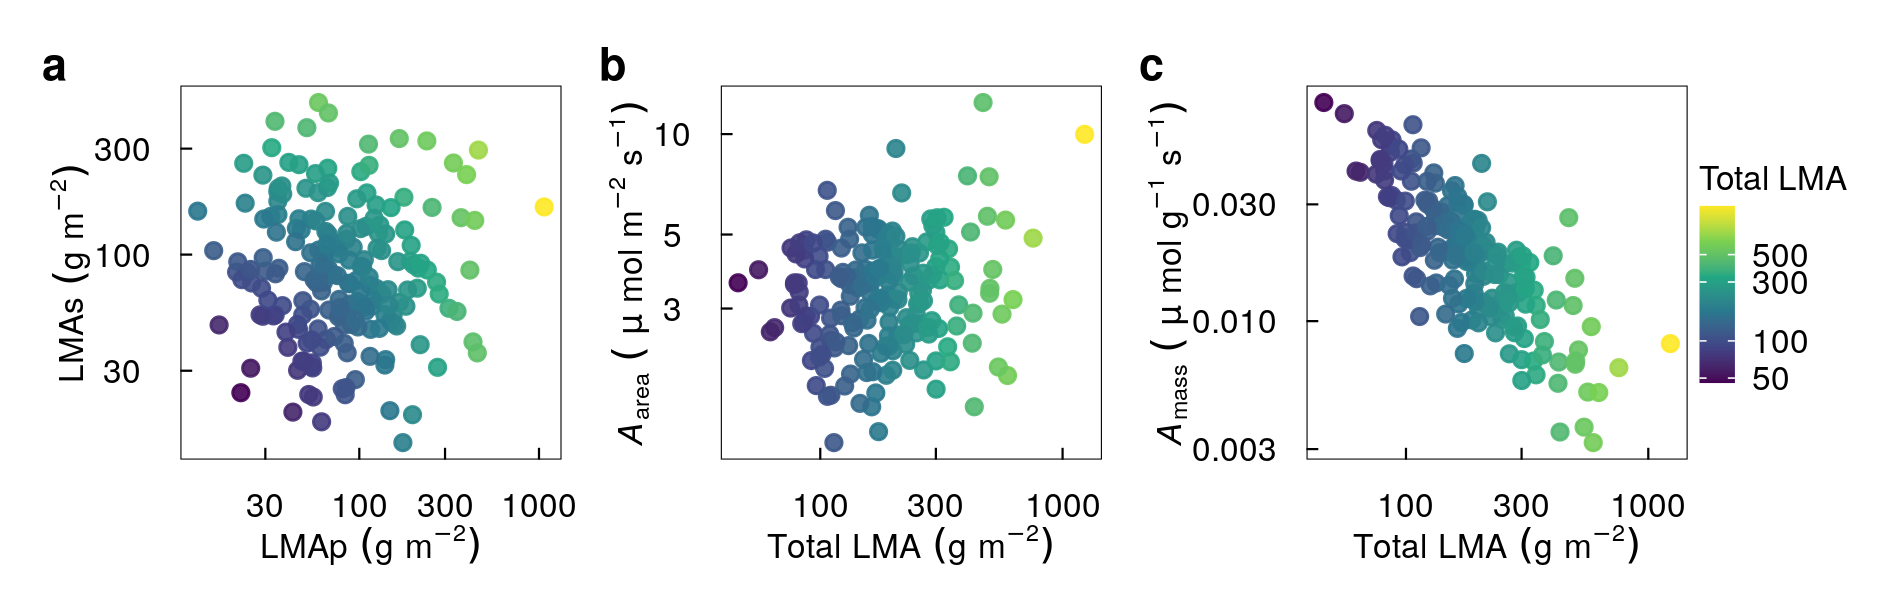
\includegraphics{../figs/hypo.png}

}

\caption{\label{fig-Hplt}Example of a two-dimensional functional space
that can result in either a two- or one-dimensional trait space,
depending on how metabolic traits are normalized. (A) Hypothetical
independent variation in two leaf mass per area (LMA) components:
metabolic leaf mass per area (LMAp, which largely determines per-area
values of photosynthesis, respiration, and nutrient concentrations) and
structural leaf mass per area (LMAs, which determines leaf toughness but
has little effect on metabolic traits). (B) Two-dimensional relationship
between photosynthetic capacity (\emph{A}\textsubscript{max}) per-unit
leaf area and total LMA (equal to LMAp + LMAs). (C) One-dimensional
relationship between \emph{A}\textsubscript{max} per-unit leaf mass and
total LMA. LMAp and LMAs are simulated from a hypothetical scenario of
lognormal distributions with medians of 80 and standard deviations of
exp(0.8) and exp(0.7), and zero covariance. Variation in
\emph{A}\textsubscript{max} values are derived from our analysis of the
GLOPNET database.
\(A_{\mathrm{area} \, i}=1.81 \times \mathrm{LMAp}_i^{0.28}\mathrm{LMAs}^{-0.13}\epsilon_i\),
where \(\epsilon_i\) is log-normally distributed with log-mean with 0,
log-scale parameter with 0.31 (see Methods and Results).}

\end{figure}

\begin{figure}

{\centering 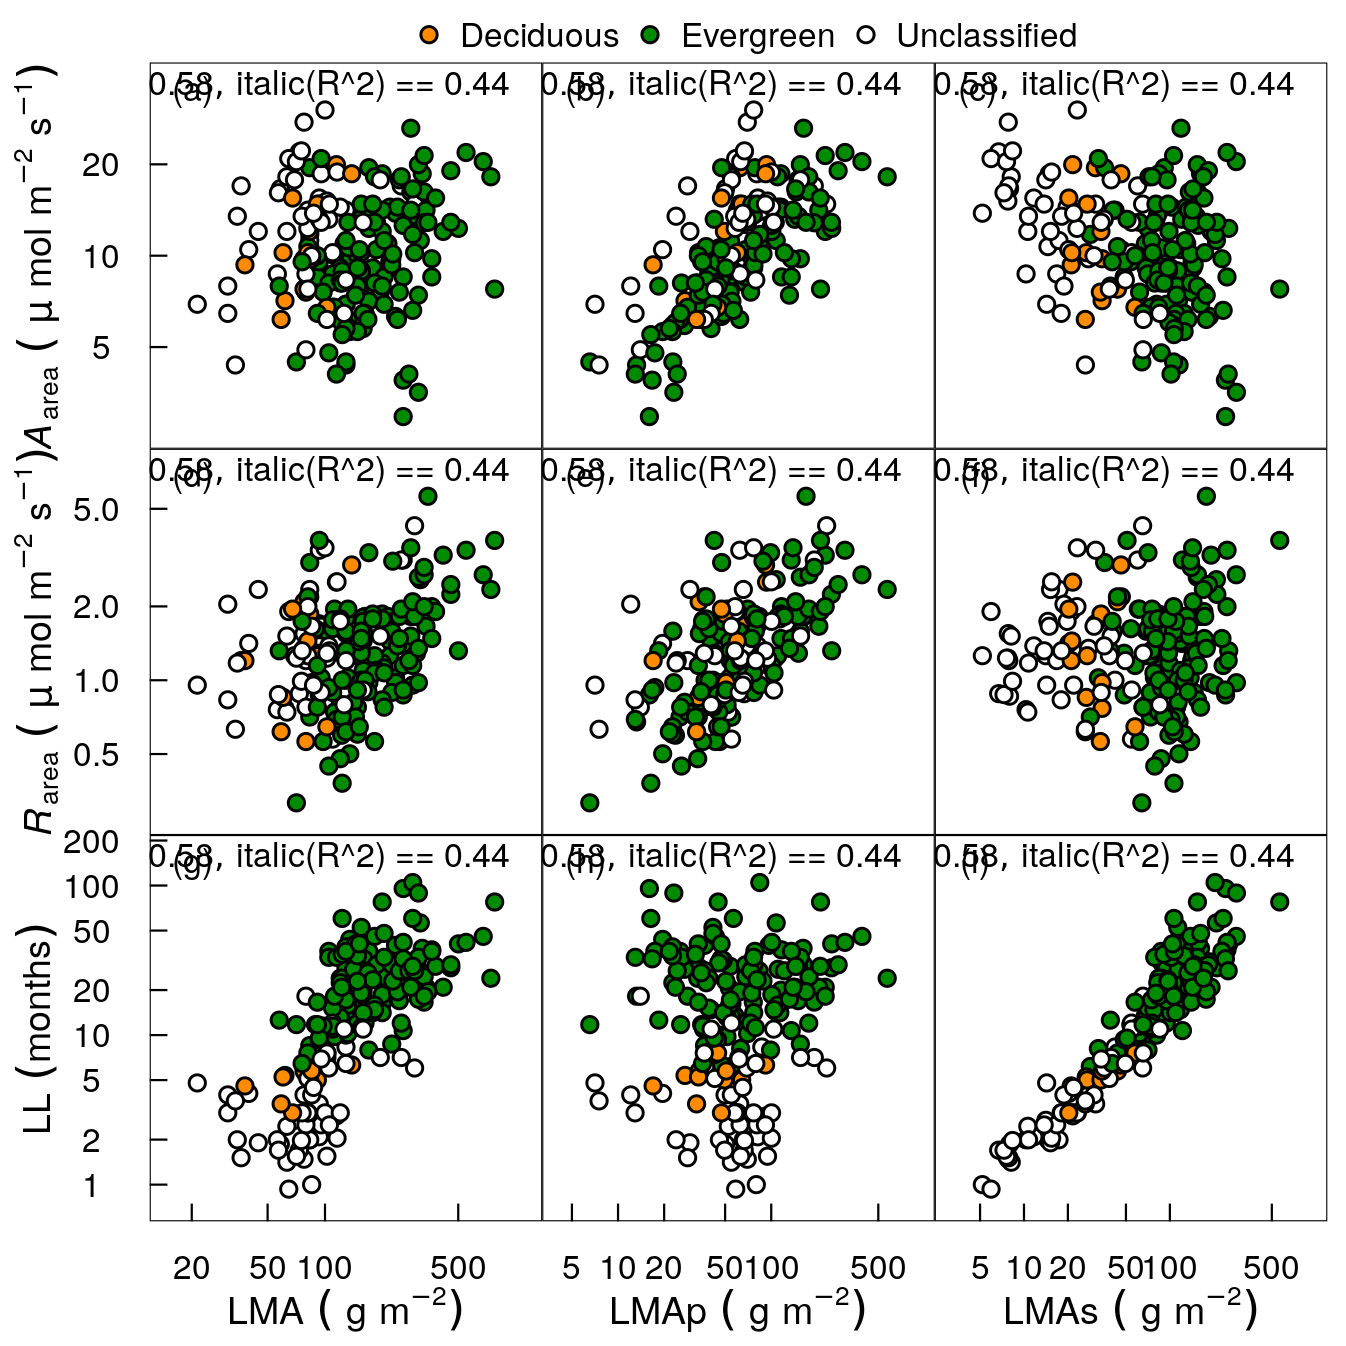
\includegraphics{../figs/gl_point.png}

}

\caption{\label{fig-GLplt}Observed and estimated leaf-trait
relationships in the global GLOPNET dataset. Estimates are from the NAME
Model (Eq. X). Leaf life span (LL), net photosynthetic rate per unit
leaf area (\emph{A}\textsubscript{area}), and dark respiration rate per
unit leaf area (\emph{R}\textsubscript{area}) are plotted against
observed LMA, posterior means of LMAp and LMAs. Pearson correlation
coefficients (\emph{r}) for LMA (left column) and posterior means of
Pearson correlation coefficients (\(\bar{r}\)) or partial correlation
coefficients (\(\bar{\rho}\)) of LMAp (middle column) and LMAs (right
column) are shown. Note that LL was modeled by LMAs alone.}

\end{figure}

\newpage

\begin{figure}

{\centering 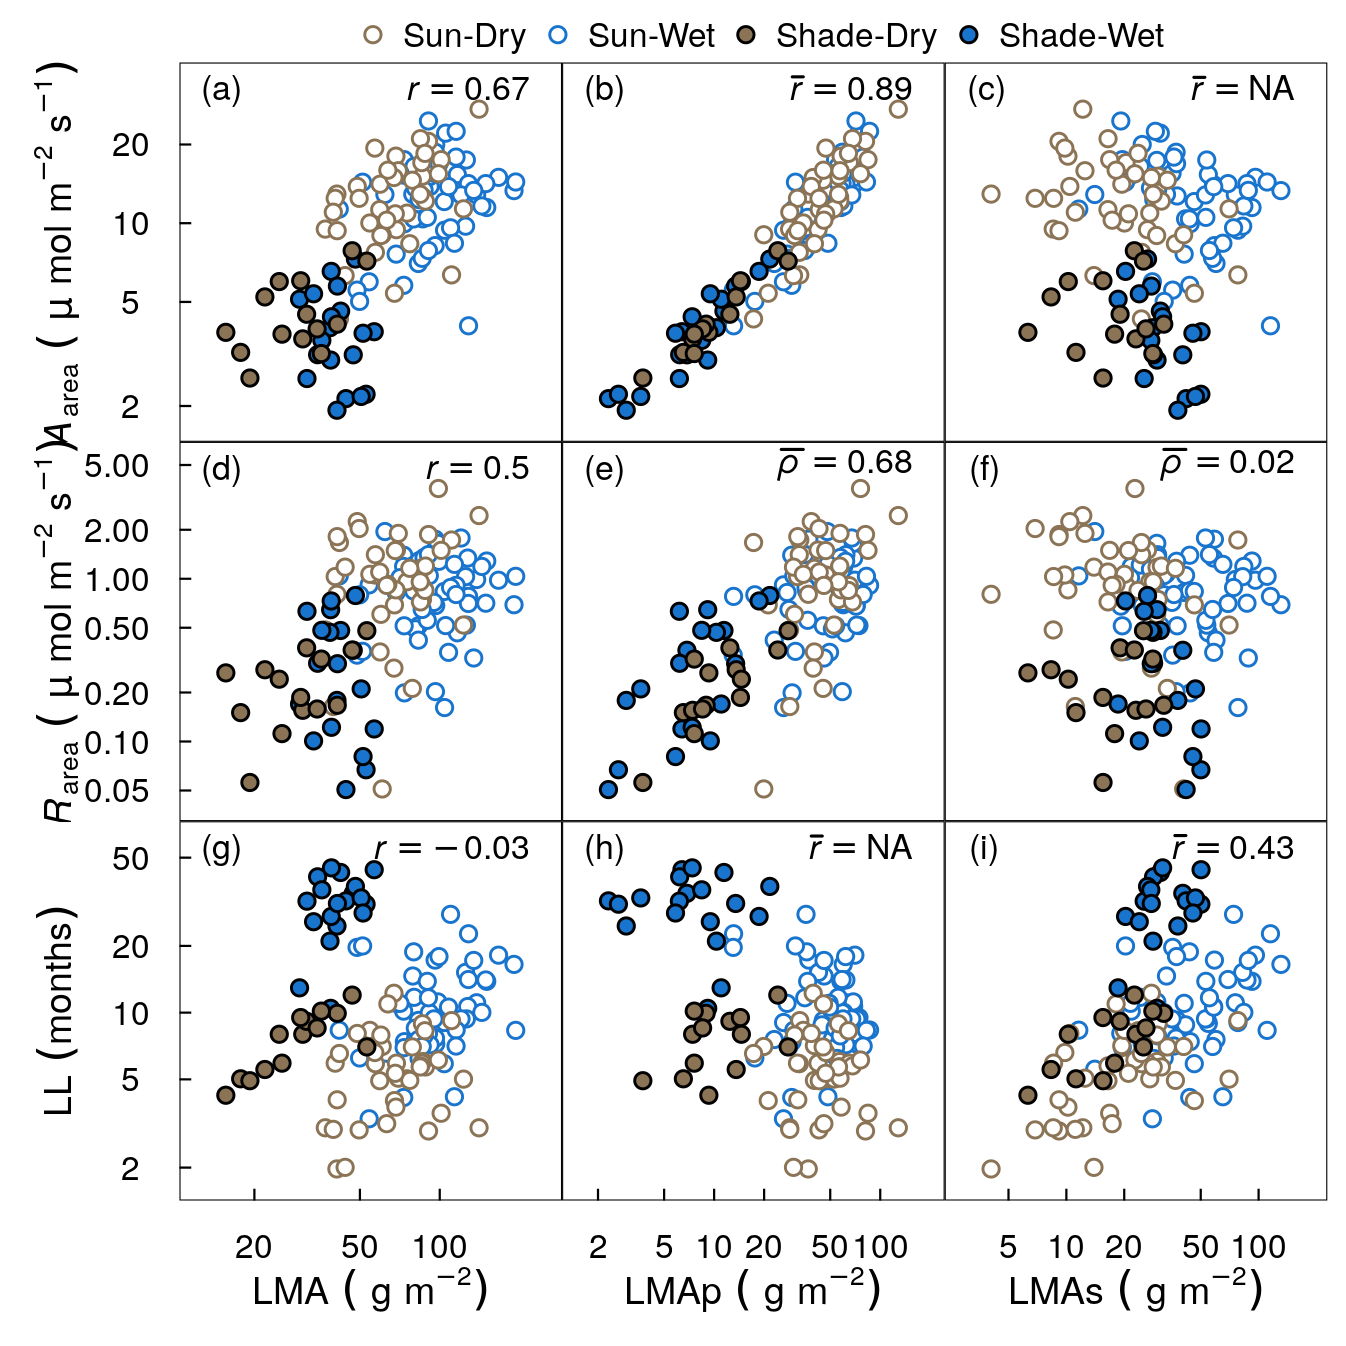
\includegraphics{../figs/pa_point.png}

}

\caption{\label{fig-PAplt}Observed and estimated leaf-trait
relationships in the Panama dataset. Estimates are from the XXX Model
(Eq. 6b). Details as in Fig.~\ref{fig-GLplt}. Results for other LL
models are summarized in Table SX. Note that
\emph{A}\textsubscript{area} and LL were modeled by LMAp and LMAs alone,
respectively.}

\end{figure}

\newpage

\begin{figure}

{\centering 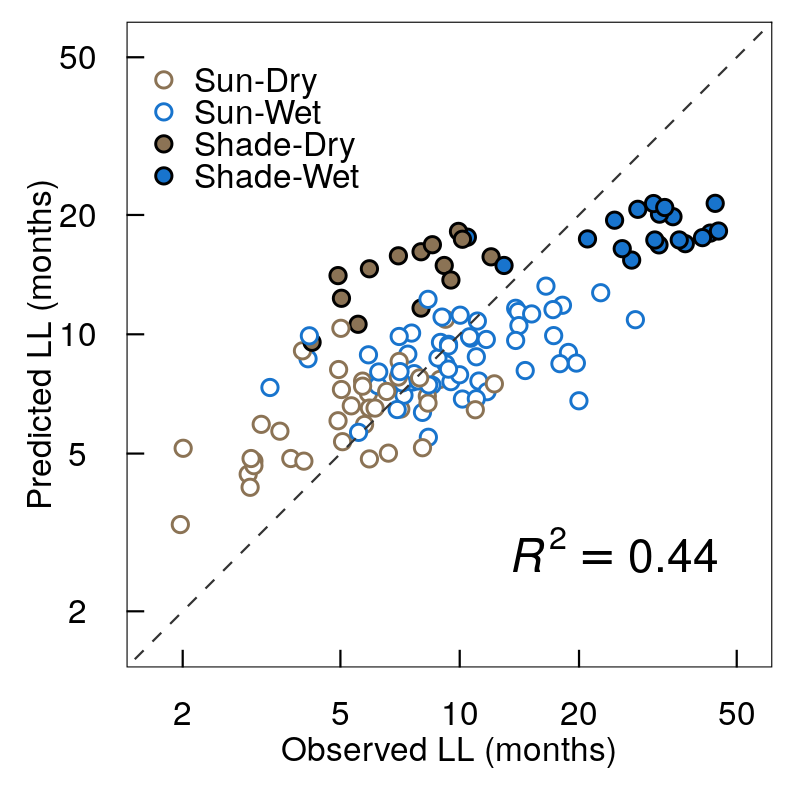
\includegraphics{../figs/pa_point_ll.png}

}

\caption{\label{fig-LLplt}Observed vs.~predicted leaf lifespan (LL) in
the LL with light Model (Eq. 6b). Predicted LL values are posterior
means. The dashed line indicates the 1:1 relationship. The
\emph{R}\textsuperscript{2} value is the posterior mean of Bayesian
\emph{R}\textsuperscript{2} (\protect\hyperlink{ref-Gelman2019}{Gelman
et al. 2019}).}

\end{figure}

\newpage

\begin{figure}

{\centering 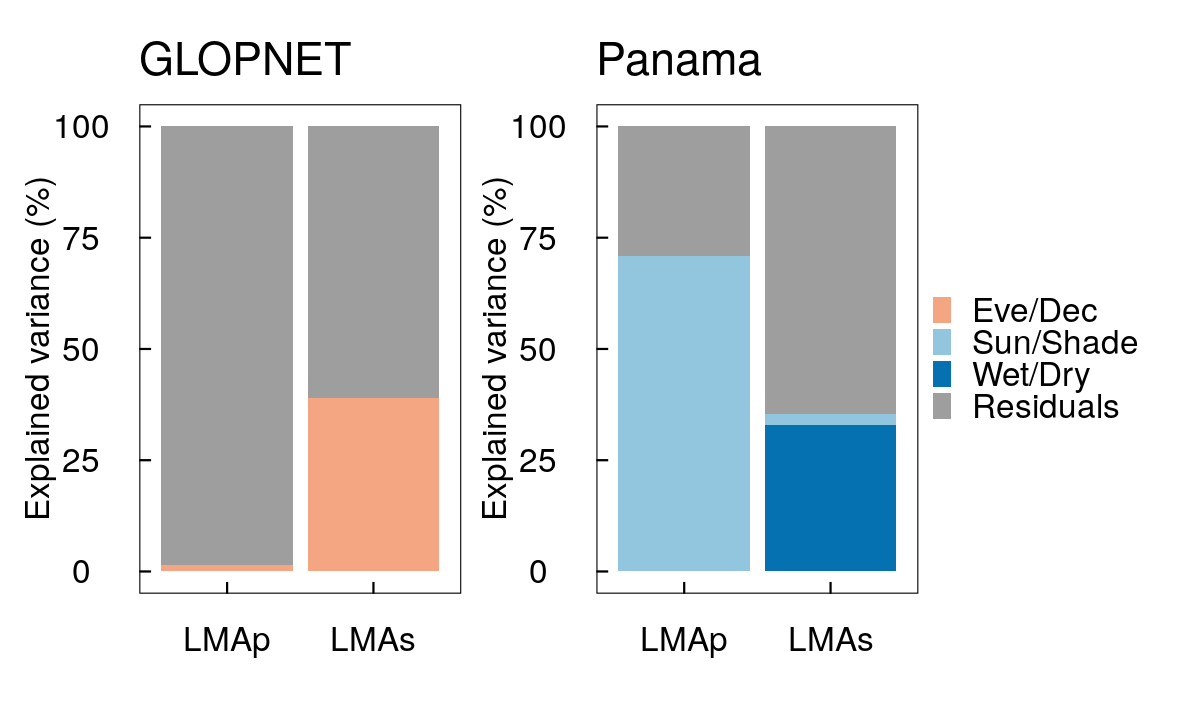
\includegraphics{../figs/vpart.png}

}

\caption{\label{fig-vpart}Variance partitioning on LMA components
between and within leaf habits (evergreen vs.~deciuous) for the GLOPNET
dataset, and between and within sites (wet vs.~dry) and light (sun
vs.~shade) for the Panama dataset.}

\end{figure}

\newpage

\begin{figure}

{\centering 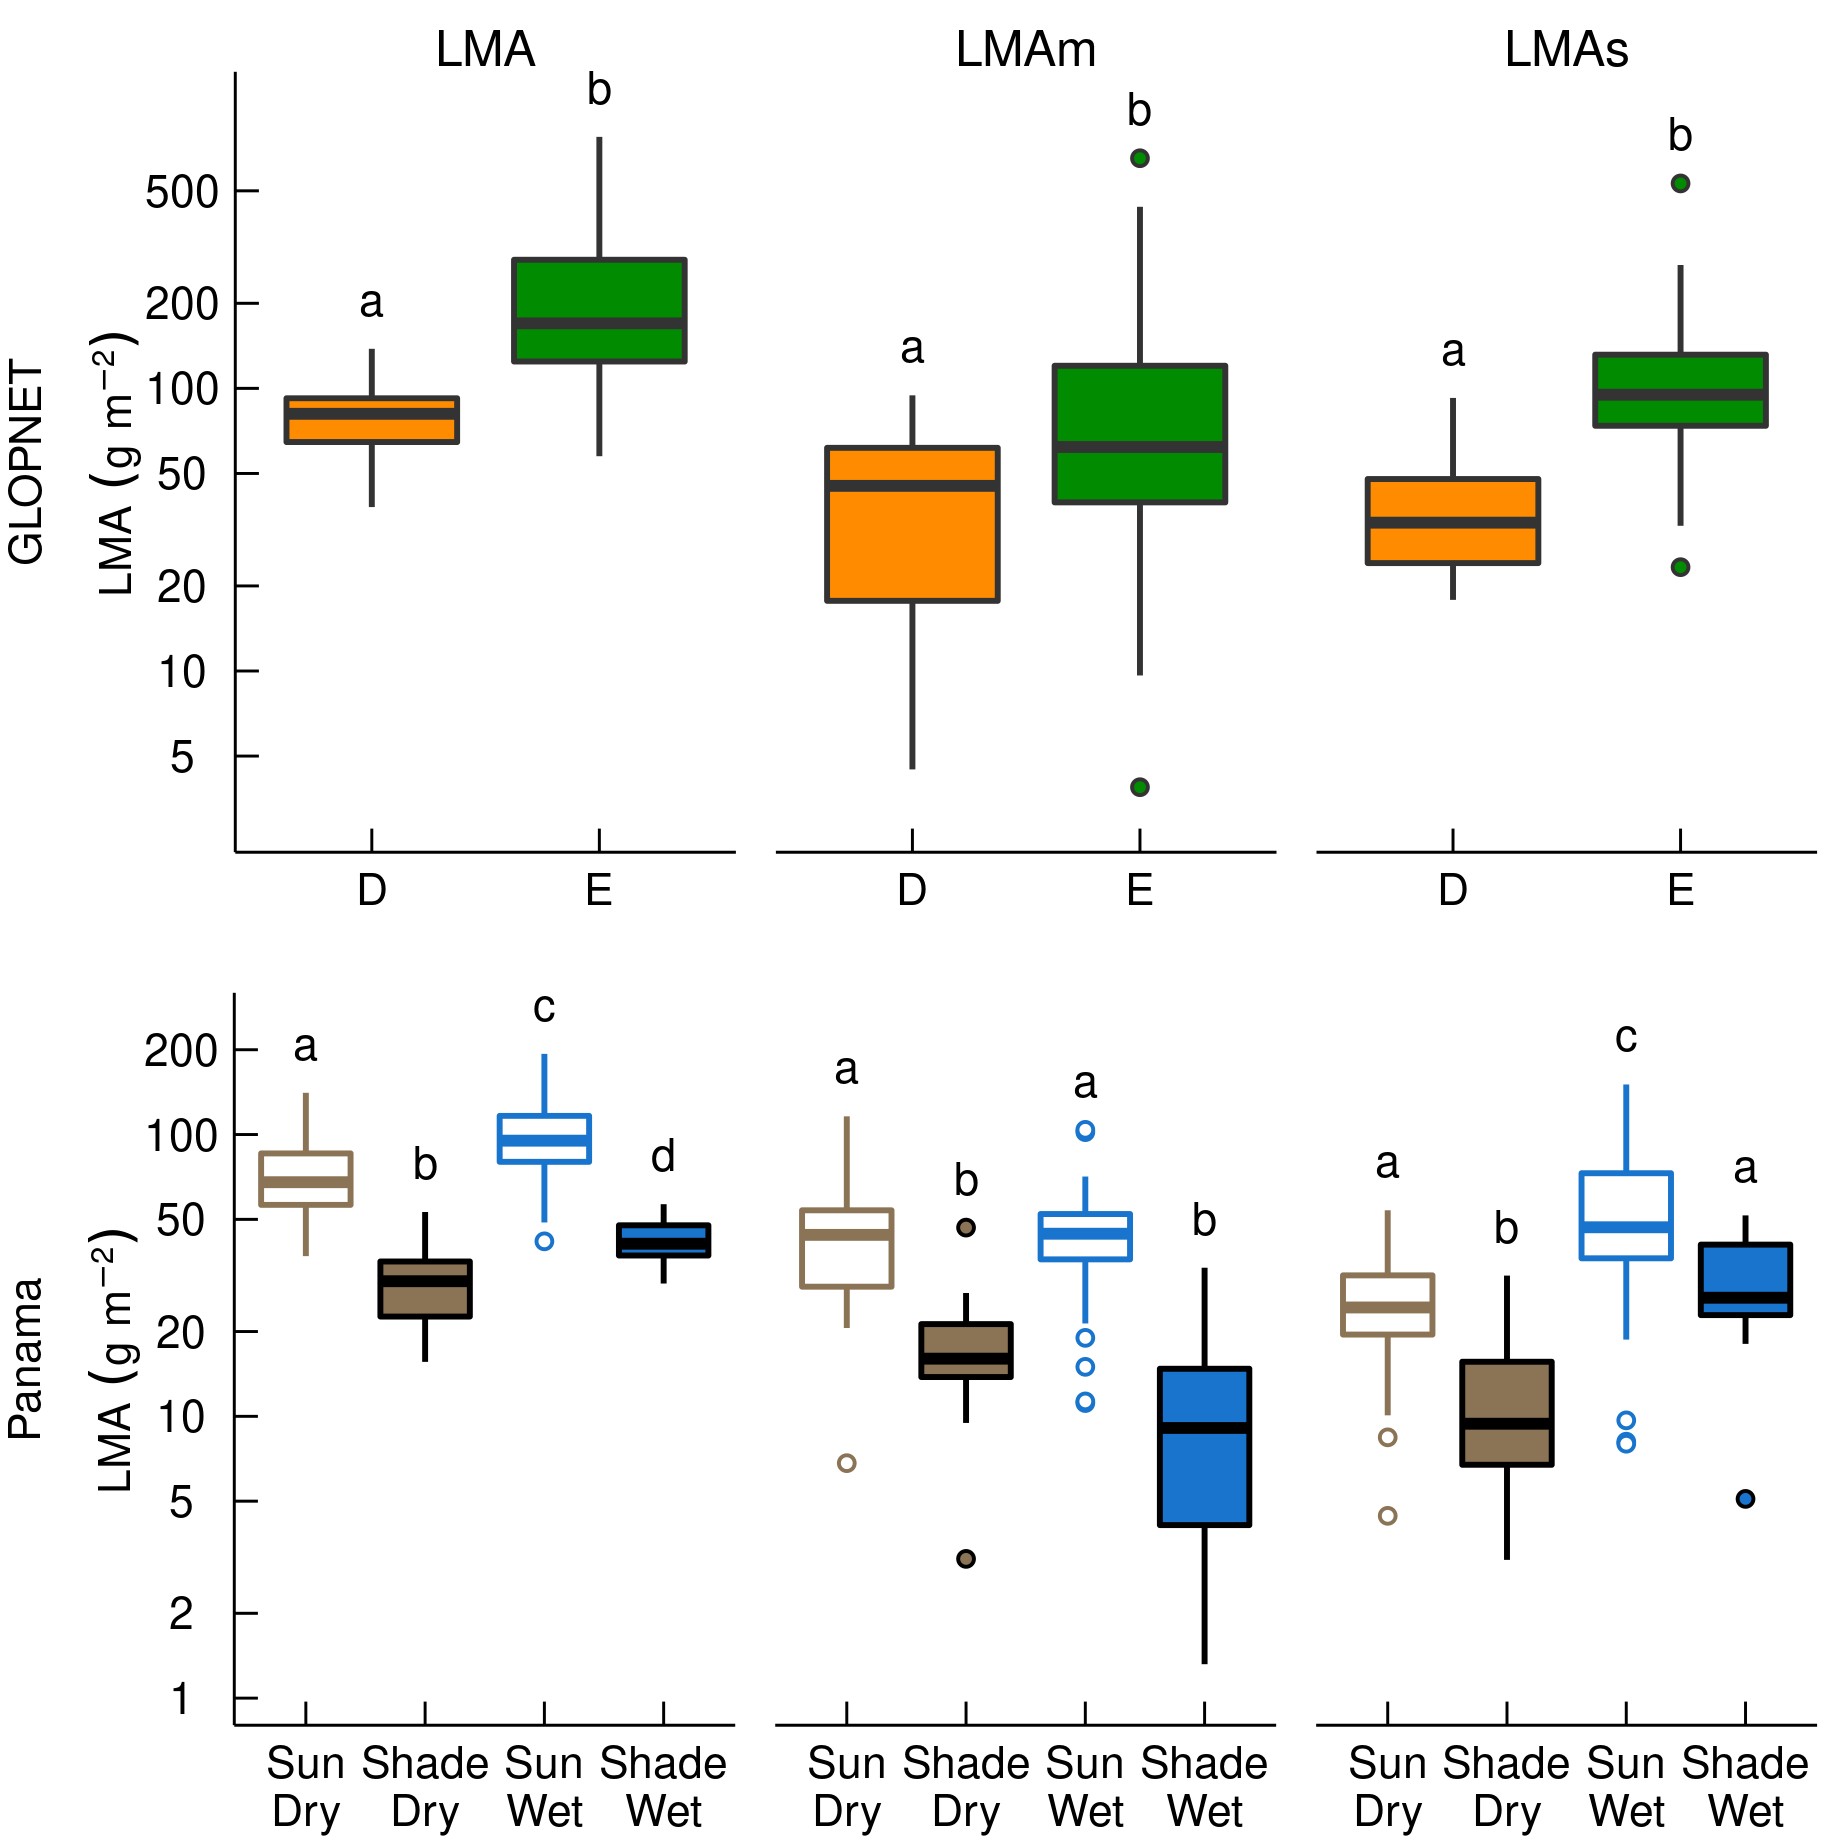
\includegraphics{../figs/box_main.png}

}

\caption{\label{fig-boxplt}Boxplots comparing leaf mass per area (LMA)
and posterior medians of photosynthetic and structural LMA components
(LMAp and LMAs, respectively) across deciduous (D) and evergreen (E)
leaves in the GLOPNET dataset (top), and across sites (wet and dry) and
canopy strata (sun and shade) in the Panama dataset (bottom). The center
line in each box indicates the median, upper and lower box edges
indicate the interquartile range, whiskers show 1.5 times the
interquartile range, and points are outliers. Groups sharing the same
letters are not significantly different (P \textgreater{} 0.05;
t-tests). To isolate the effects of intraspecific variation (i.e.,
plastic responses to light), the Panama results shown here only include
species for which both sun and shade leaves were available.
Qualitatively similar results were obtained when all Panama species were
included (Fig. SX). Note that the vertical axis is on a
log\textsubscript{10} scale.}

\end{figure}

\newpage

\begin{figure}

{\centering 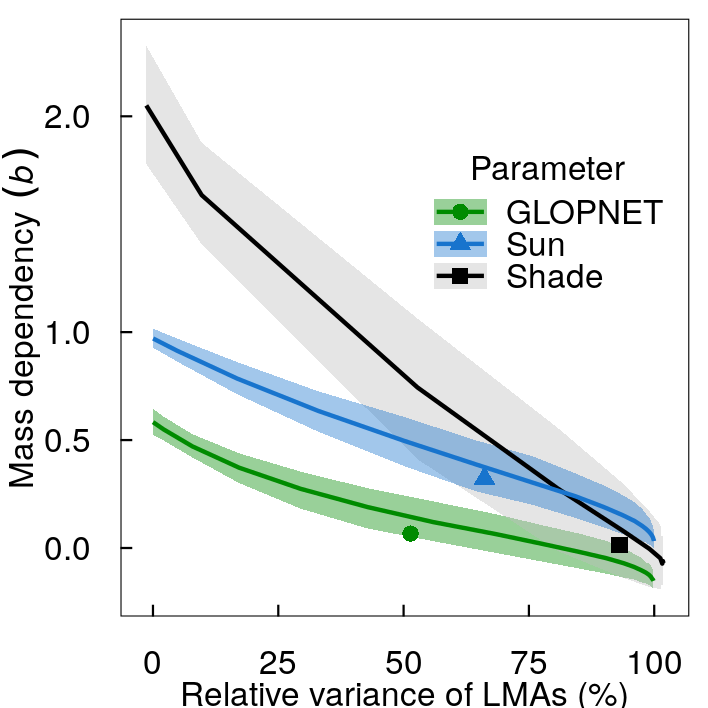
\includegraphics{../figs/mass_prop_mv.png}

}

\caption{\label{fig-massplt}The relationships between mass dependency
(\emph{b} in Eq. 8) and relative variance in LMAs to LMA for the global
GLOPNET dataset, sun leaves in Panama, and shade leaves in Panama. Solid
lines indicate simulated means and shaded regions indicate 95\% CI. Each
symbol indicates the estimated values from the empirical data. The
photosynthetic rate (\emph{A}\textsubscript{max}) is primarily
mass-dependent (\emph{b} \textgreater{} 0.5), primarily area-dependent
(0.5 \textgreater{} \emph{b} \textgreater{} 0) and purely area-dependent
(\emph{b} = 0) (\protect\hyperlink{ref-Osnas2018}{Osnas et al. 2018}).
Note that when \emph{b} \textgreater{} 1, \emph{A}\textsubscript{area}
dramatically increases with LMA, which is not realistic.}

\end{figure}

\newpage

\begin{figure}

{\centering 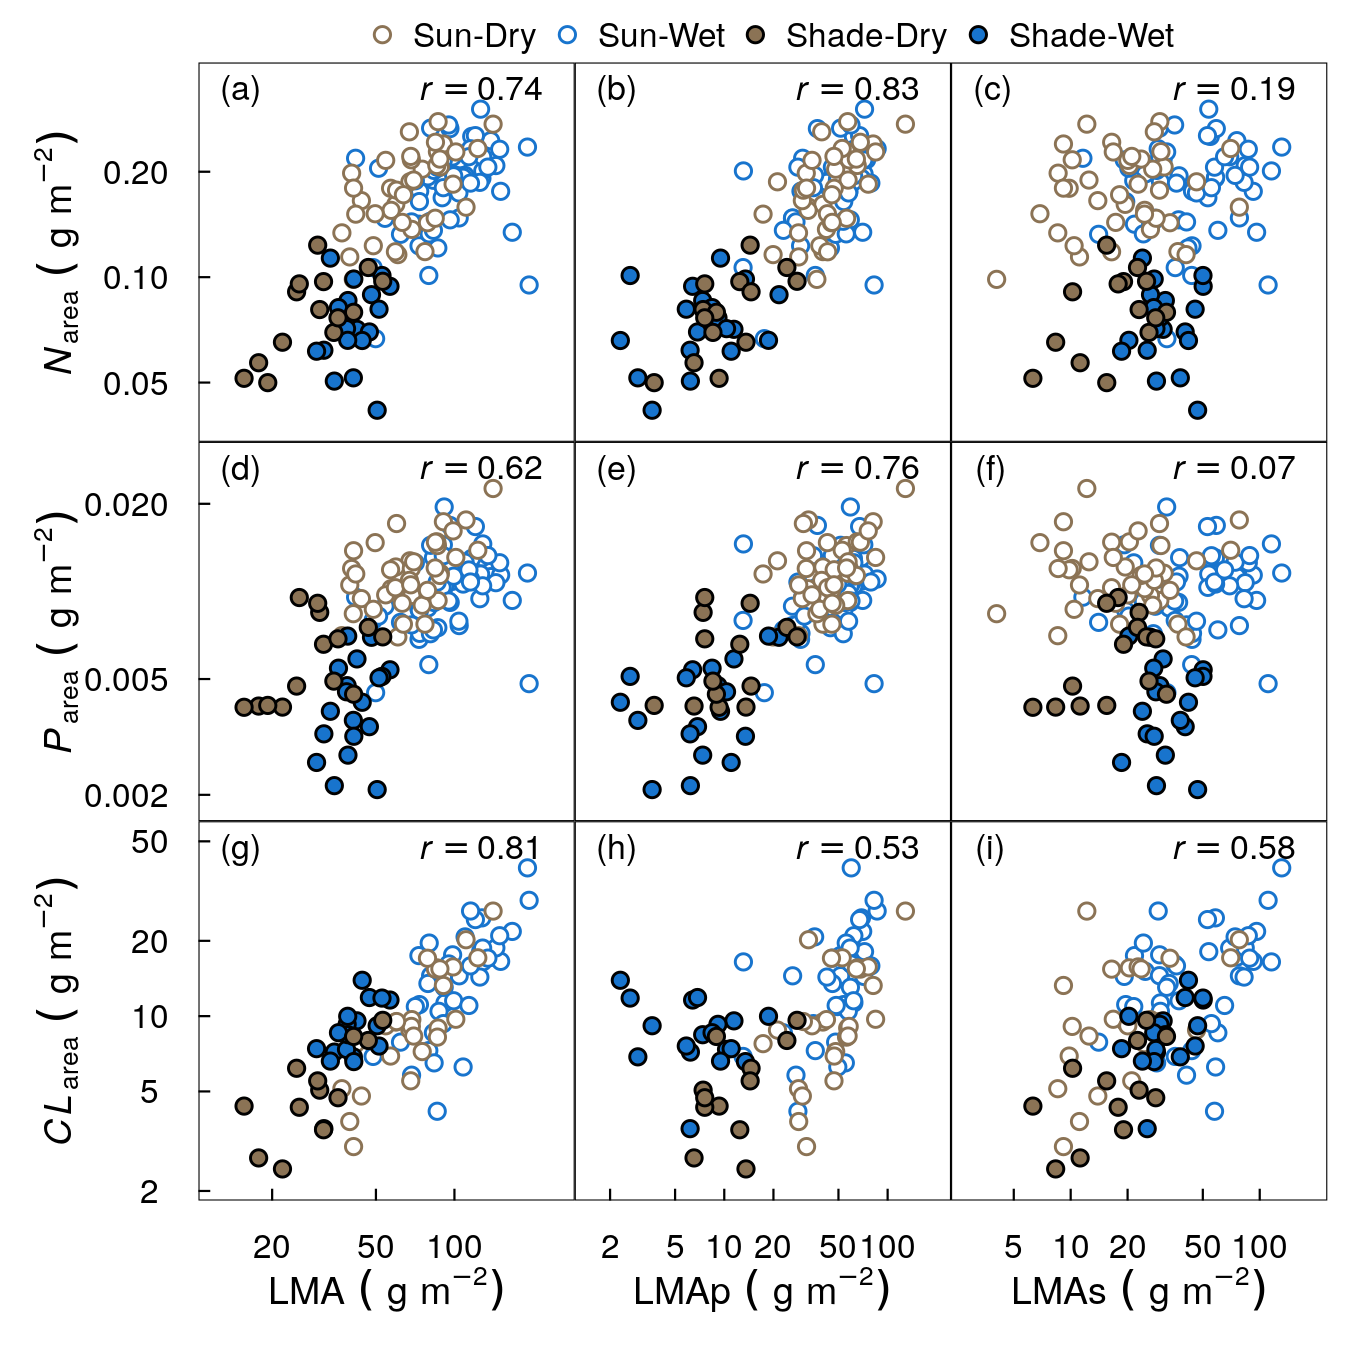
\includegraphics{../figs/pa_point_npc.png}

}

\caption{\label{fig-PA-NPC}Measured traits related to photosynthesis and
metabolism traits (nitrogen and phosphorus per-unit leaf area;
\emph{N}\textsubscript{area} and \emph{P}\textsubscript{area}) are
strongly correlated with estimates (posterior medians) of the
photosynthetic LMA component (LMAp), and a measured structural trait
(cellulose per-unit leaf area; \emph{CL}\textsubscript{area}) is
strongly correlated with estimates of the structural LMA component
(LMAs) for the Panama dataset. Note that sun and shade leaves align
along a single relationship for \emph{CL}\textsubscript{area} vs.~LMAs,
but not for \emph{CL}\textsubscript{area} vs.~LMA or LMAp.
\emph{N}\textsubscript{area}, \emph{P}\textsubscript{area}, and
\emph{CL}\textsubscript{area} data were not used to fit the models, and
are presented here as independent support for the model results. Pearson
correlation coefficients (\emph{r}) for LMA (left column) and partial
correlation coefficients (\(\rho\)) of LMAp (middle column) and LMAs
(right column) are shown. Analogous results were obtained for
\emph{N}\textsubscript{area} and \emph{P}\textsubscript{area} for
GLOPNET (Fig. S3). Results for other LL models are reported in Table
SX.}

\end{figure}

\end{document}
